\documentclass[a4paper,12pt]{book}

\usepackage{amsmath}
\usepackage[top=1.0in,bottom=1.0in,left=1.5in,right=1in]{geometry}
\usepackage{epstopdf}
%\usepackage{hyperref}


\usepackage{amssymb}
\usepackage{graphicx}
\usepackage{braket}
\usepackage{cases}
\usepackage{paralist}
\usepackage{eufrak}
\usepackage{amscd}

%% Page Style
\usepackage{fancyhdr}
\pagestyle{fancy}
\renewcommand{\chaptermark}[1]{\markboth{\chaptername\ \thechapter.\ #1}{}}
\renewcommand{\sectionmark}[1]{\markright{\thesection.\ #1}}
\newcommand{\helv}{\fontfamily{phv}\fontseries{n}\fontsize{12}{12}\selectfont}

\fancyhf{}
\fancyhead[LE]{\helv \nouppercase{\rightmark}}
\fancyhead[LO]{\helv \nouppercase{\leftmark}}
\fancyfoot[RO,RE]{\thepage}
\renewcommand{\headrulewidth}{0pt}
\renewcommand{\footrulewidth}{0pt}
\fancypagestyle{plain} {
\fancyhead{} % get rid of headers
}

\usepackage{indentfirst}
%%\linespread{2.0}

\def\bE{{\mathbb{E}}}
\def\bR{{\mathbb{R}}}

\def\eqlaw{{\stackrel{\text{(law)}}{=}}}
\def\tS{{\widetilde{S}}}
\def\tB{{\widetilde{B}}}
\def\tmu{{\widetilde{\mu}}}
\def\tsigma{{\widetilde{\sigma}}}
\def\abs#1{{\left|#1\right|}}
\def\E{{\mathrm{E}\,}}
\def\EE#1{{{\mathrm{E}}\left(#1\right)}}


\def\tX{{\widetilde{X}}}
\def\tM{{\widetilde{M}}}
\def\tx{{\widetilde{x}}}
\def\tm{{\widetilde{m}}}

\def\M{{\mathcal{M}}}

\allowdisplaybreaks[1]
 
\usepackage{natbib}


\usepackage{hyperref}

\usepackage{titletoc}

\contentsmargin{2.55em}
\titlecontents{section}
	[3.5em]
	{\vspace{\baselineskip}}
	{\contentslabel{2.3em}}
	{\hspace*{-2.3em}}
	{\titlerule*[1pc]{.}\contentspage}

\titlecontents{subsection}
	[5.8em]
	{\vspace{\baselineskip}}
	{\contentslabel{3.2em}}
	{\hspace*{-3.2em}}
	{\titlerule*[1pc]{.}\contentspage}

\titlecontents{figure} 
	[2em]
	{}
	{\contentslabel{2.3em}}
	{\hspace*{2.3em}}
	{\titlerule*[1pc]{.}\contentspage\vspace{\baselineskip}}

\titlecontents{table} 
	[2em]
	{}
	{\contentslabel{2.3em}}
	{\hspace*{2.3em}}
	{\titlerule*[1pc]{.}\contentspage\vspace{\baselineskip}}

	
\usepackage{setspace}

\begin{document}
\bibliographystyle{mycje}
\frontmatter

%% title page
\thispagestyle{empty}
\vspace{2cm}
\begin{center}\Large \bf
On Quantiles of Brownian Motion and Quantile Options

\vfill

Zhu Yong Ting

\textit{(B.Sc., Soochow University)}

\vfill

\normalsize
A THESIS SUBMITTED

\vspace{1em}

FOR THE DEGREE OF MASTER OF SCIENCE

\vspace{1em}

DEPARTMENT OF STATISTICS 

\vspace{1em}

AND APPLIED PROBABILITY

\vspace{1em}
\large
NATIONAL UNIVERSITY OF SINGAPORE

\vspace{1em}

2009

\end{center}

\vspace*{1cm}

\pagebreak

%\renewcommand{\baselinestretch}{2}
\doublespacing
\normalsize


\chapter{Acknowledgements}




%\renewcommand{\baselinestretch}{1}
\singlespacing
%\pagestyle{fancy}
%\pagenumbering{roman}
\setcounter{tocdepth}{3}
\tableofcontents 

%\renewcommand{\baselinestretch}{2}
\doublespacing

\chapter{Abstract}
Option is the one popular derivative traded in market. 
%So evaluate the value of options is
%a very important question in finicial industry.
%However the return of options can only be determined when it is exercised.
%So option pricing became a very difficult problem.
In the most important model, Black-Scholes model, for option pricing, 
the price of underling asset is assumed to 
satisfy the geometric Brownian motion, 
which is a very interesting object itself. 
We will have a quick review about the theory of option pricing
in the fist part of this thesis.
%So option priceing is a  very interesting and important problem
%both in practical and theratical. 
It is well known that Black-Scholes formula solves pricing problem 
for European option.
However, for other types of options, usually there is no such nice formula. 
Numerical methods are developed to solve these problems. 
In this thesis, we consider the $\alpha$-quantile options. 
Partially because the $\alpha$-quantiles of Brownian motion 
are highly path-dependent, many fundamental problems are still open.
One problem is the discretization error between the $\alpha$-quantile 
of Brownian motion and that of Gaussian random walk. 
This is the first step to find the order of approximation for numerical 
methods based on Gaussian random walk.
We have found a big difference between the
convergence patterns of the discrete error for genuine $\alpha$-quantiles $(0< \alpha < 1)$
and the maximum ($\alpha=1$) by simulation. 
Moreover we show these differences theoretically.
Another problem is using tree methods to price 
$\alpha$-quantile options. A forward shooting method for European-style $\alpha$-quantile option originally proposed by \cite{Kwok2001} are studied. We propose a tree method which can price both European and American-style of $\alpha$-quantile options. Richardson extrapolation is applied to accelerate the convergence speed of our lattice method. 
\vspace{1cm}

\noindent{\bf Keywords}: Option Pricing, $\alpha$-quantile Options, Discretization error, Tree Method, American option, Optimal Stopping Problem, Richardson Extrapolation


%\renewcommand{\baselinestretch}{1}
\singlespacing

\listoftables 
\listoffigures
\indent

\mainmatter

%\renewcommand{\baselinestretch}{2}
\doublespacing
\small\normalsize

\chapter{Introduction}
\pagenumbering{arabic}


\cite{Hull2008} defines an {\it option} to be a contract which provides the holder the right to buy or sell an underlying asset at or before a certain date at a predetermined price. The price determined in the contract is called the {\it strike price}. To get this right, the buyer should pay the seller. Every option contract involves two sides of investors. One side is known as the long side. On the long side is the investor who has bought the option.  Another side is called the short position who has sold the option. If the long side chooses to exercise the right defined in the contract, the short side has the obligation to perform the transaction with the long side at the specified price set in the contract. Since there exists a disparity of right and obligation, the long side should pay a premium to the short side to obtain this right. However, this contract is only in effect before a certain date. This date set in the contract is called the {\it expiration date} or {\it maturity}. Basically, there are two types of option contracts. A holder of a {\it call} option has the right to buy the underlying asset at the predetermined price, while a holder of a {\it put} option has the right to sell the underlying asset at the predetermined price. European options can be exercised only at the expiration date. American options on the other hand can be exercised at any time before the expiration date.

To help the understanding of options, here we give an example of the use of an option. Suppose that it is now January 15. A copper fabricator expects it will need 100,000 pounds of copper on May 15 to meet a certain contract. The spot price of copper is 140 cents per pound. To fix the expense of raw material, the fabricator may take a long position of a call option, for example, a call option with a strike price of \$120,000 for 100,000 pounds of copper expiring in four months. Holding this option, the fabricator eliminates its risk exposure to the changes of copper price. This example shows an option being used as a hedging instrument. There are other purposes of using options.

Generally, there are three broad categories of traders of options: {\it hedgers}, {\it speculators}, and {\it arbitrageurs}. Hedgers are the group of investors who use options to reduce the risk associated with potential future movements of the price for a certain asset. Speculators bet on the future direction of an asset using options. Taking advantage of a discrepancy between prices in two different markets, arbitrageurs lock in risk-free profits by concurrently taking offsetting positions in two or more markets. One main reason contributing to the success of option markets is that they meet the needs of different types of traders.

Options have a long history. There is evidence that Romans and Phoenicians used similar contracts in shipping. In ancient Greece, a famous mathematician and philosopher, Thales, used options to obtain a low price for olive presses ahead of the harvest. In the 17th century the Dutch bought and sold options structured on tulip. However, the trading of options actually took off in the 1970s. The Chicago Board of Trade established the Chicago Board Options Exchange (CBOE) and began trading listed call options on 16 stocks on April 26, 1973. From then, innovation has bred the creation of copious products tailored to meet the needs of different types of investors. Exotic options, such as Asian options, barrier options and lookback options are traded routinely. One common character of these exotic options is that they are usually path-dependent. 
Recently, even more exotic types of options such as Parisian options and ${\alpha}$-quantile options have appeared and attracted interest. Although exotic options are a relatively small part of the financial market in terms of volume, these options are important to investment banks because they are generally much more profitable than plain vanilla options.

Options are bought and sold in two ways. Options with standardized terms are traded on organized exchanges. These kinds of options are more standard and liquid than over-the-counter options. Over-the-counter options are not listed in exchanges and instead are only quoted by financial institutions. According to the statistics published by the Bank for International Settlements, the central bankers' central bank, in June $2009$, the amounts outstanding on options traded in organized exchanges were $\$43.75$ trillion and the figure for over-the-counter options was $\$68.19$ trillion.

The prosperity of option markets calls for valuation methods of options. While in return, the success of pricing model also boosts the development of options. In Chapter $2$, we review the fundamental pricing principles for both European and American options. Popular numerical methods are outlined in Chapter $3$. In Chapter $4$, we give an extensive study of quantiles of Brownian motion and quantile options. This is the main focus in this thesis.

\chapter{Principles of option pricing}

% add more Brodie option pricing: valuation models and applications and the
In general, the price of a stock option is influenced by five factors:
\begin{enumerate}[1.]
\item The spot stock price, $S_t$
\item The strike price set in the contract, $K$
\item The remaining time to maturity, $T-t$, where $T$ is the maturity of the option
\item The volatility of the underlying stock price, $\sigma$
\item The risk-free interest rate, $r$
\end{enumerate}

Because a holder of an option contract has the right but not an obligation to exercise the option, the payoff of an option is always non-negative. For a European option, the exercise payoff from a long position is $(S_T - K)^+ = \max \{S_T-K,0\}$. As for an American option, the payoff function is similar; what is different is that we should use the spot stock price $S_t$ when the option is exercised to calculate the payoff, instead of $S_T$ in the European case. 

In many cases there are closed-form pricing formulas for European options. In addition, numerical approaches such as the binomial tree and Monte Carlo simulation can solve this problem. We give a brief overview of these numerical methods in Chapter $3$. Because we do not know when an American option will be exercised, the pricing of American options is more complicated. A complete solution to an American option pricing problem should address two aspects, option value and an optimal exercise strategy. However, only in a few cases are analytic solutions available. In most cases, a numerical approach is needed. For example, \cite{Lim2004} proposed an approach to compute both the price and the optimal exercise boundary for American-style lookback options.

In this chapter, we review the two major option pricing principles, no-arbitrage valuation and risk-neutral valuation. The valuation of American options is also discussed. We refer the reader to \cite{2004Broadie} for a more exhaustive review of option valuation models and applications. Since lookback options are special cases of $\alpha$-quantile options with $\alpha = 1$, the pricing methods of lookback options are summarized. 

\section{European options}
\subsection{No-arbitrage valuation}

Absence of arbitrage is the fundamental principle of option pricing. \citet*{Black:1973} provided the landmark paper in the field of option pricing. \citet*{merton1973} was the first to extend this valuation model to incorporate dividend payments. In his paper, the rationality of option pricing was also discussed. 

%\subsubsection{Black-Scholes framework}
The Black-Scholes model is one of the most extensively used models to describe stock price behavior.
Let $S_t$ be the stock price. Then under this model, $S_t$ satisfies 
\begin{equation}\label{eq:1}
dS_t = \mu S_tdt + \sigma S_tdB_t,
\end{equation}
with $\mu$ and $\sigma $ constant, which represent the expected return on the stock and the volatility respectively. The process $\{B_t\}$ is a standard Brownian motion on probability space $(\Omega,\mathcal{F}, \mathbb{Q})$ which represents the underlying uncertainty of the market. With initial stock price $S_0$ at time $0$, the solution to (\ref{eq:1}) is 
\begin{equation}
S_t=S_0\exp((\mu-\sigma^2 /2)t + \sigma B_t)
\end{equation}
Thus the stochastic process $S_t$ is also knownn as a geometric Brownian motion (GBM). 

There are other assumptions in this model as follows:

\begin{enumerate}[1.]
\item Investors are able to borrow and lend cash at the same risk-free interest rate $r$. This risk-free interest rate is known and constant. 
\item There are no transaction fees.
\item There are no tax costs. 
\item The stock does not pay a dividend. 
\item Investors can buy any fraction of a share. 
\item Short selling is allowed without limitations and restrictions. 
\item The market is absent of arbitrage opportunities. That is, no one can profit from nothing.  
\item Securities trade continuously. This means you can sell or buy a security at any time.
\end{enumerate}

These assumptions are usually referred to as the Black-Scholes framework. Further studies show that many conditions can be relaxed. For simplicity, we follow the Black-Scholes framework in this section.

% This approach to model stock price was first introduced by Black, Scholes and Merton.
% Denote $r$ as the constant continuously compounded risk-free interest rate. Under risk-neutral assumption, we can get $\mu = r $.

%\subsubsection{Black-Scholes PDE}
Let $V(S, t)$ be the price of a European vanilla option at time $t$ when the stock price is $S$. The value $V(S,T)$ at maturity $T$ is the payoff. Suppose $V(S,t)$ is twice differentiable, applying It\^o's formula (\cite{Steven}~(4.4.24)) to $V$ we get
\begin{equation}\label{ito}
dV_t = \left( \frac{\partial V}{\partial t} + \frac{\partial V}{\partial S} S_t \mu + \frac{1}{2}\frac{{\partial}^2V}{\partial S^2} {S_t^2} {\sigma}^2 \right) dt + \frac{\partial V}{\partial S} S_t \sigma d B_t,
\end{equation}
where $V_t = V(S_t,t)$. The partial derivatives in (\ref{ito}) and in the sequel are evaluated at $(S_t,t)$.

More precisely, a stochastic process $X_t$ is called an It\^o process (\cite{Steven}~Definition~4.4.3) if
\[
dX_t = \mu_t dt +\sigma_t dB_t,
\]
where $\mu_t$ and $\sigma_t$ are adapted stochastic processes 
satisfying $E(\int_0^t \sigma_u^2 du) <\infty$ and $\int_0^t |\mu_u|du<\infty$ for any $t>0$.

For any function $f(x,t)$ with continuous partial derivatives 
$\partial{f}/\partial t, \partial f/\partial x$ and $\partial^2 f/\partial x^2$,
 $f(X_t,t)$ is an It\^o process satisfying
\[
d f(X_t,t) = \frac{\partial f}{\partial t}(X_t,t) dt +\frac{\partial f}{\partial x}(X_t,t) dX_t
+ \frac{1}{2} \frac{\partial^2 f}{\partial x^2}(X_t,t) \sigma_t^2 dt.
\]
Since the stochastic process $S_t$ is an It\^o process. Applying the above result we get equation~(\ref{ito}).

As $V_t$ and $S_t$ share the same underlying uncertainty, we can eliminate Brownian motion $B_t$ by constructing a certain portfolio with stocks and options. The appropriate trading strategy is holding one option and $-{\partial V}/{\partial S}$ shares of stock.

At time $t$, the value of this portfolio is
\begin{equation}
\Pi_t = V_t - \frac{\partial V}{\partial S} S_t.
\end{equation}

The instantaneous profit or loss $d\Pi_t$ over time interval $[t, t+dt]$ is
\begin{equation}\label{dR}
d\Pi_t = dV_t - \frac{\partial V}{\partial S} dS_t.
\end{equation}

Substituting equations (\ref{eq:1}) and (\ref{ito}) in (\ref{dR}), we get
\begin{equation}\label{dR2}
d\Pi_t= \left(\frac{\partial V}{\partial t} + \frac{1}{2}\frac{{\partial}^2 V }{\partial S^2} S_t^2 {\sigma}^2 \right) dt.
\end{equation}

Equation (\ref{dR2}) does not contain $dB_t$, which means that the return of the portfolio is entirely riskless. Since we suppose the market is absent of arbitrage, the rate of return on this portfolio must be the same as  the risk-free rate. If the return rate of the portfolio $\Pi$ is larger than the risk-free rate, an investor can borrow at the risk-free rate to go long on the portfolio. By this strategy, a investor can instantly make a profit from nothing. If the return rate of portfolio is smaller than risk-free rate, a investor can short the portfolio and invest the money at the risk-free rate. Then again the investor can make a profit from nothing. To eliminate the opportunity of arbitrage, the return rate of the riskless portfolio must be equal to the risk-free rate $r$. Then over time period $[t, t + dt]$ we have
\begin{equation}\label{dR3}
r \Pi dt = d\Pi_t =  \left(\frac{\partial V}{\partial t} + \frac{1}{2}\frac{{\partial}^2}{\partial S^2} S_t^2 {\sigma}^2 \right) dt.
\end{equation}

From (\ref{dR3}), we then get the Black-Scholes partial differential equation (PDE):
\begin{equation}\label{black-pde}
\frac{\partial V}{\partial t} + \frac{\partial V }{\partial S} S r + \frac{1}{2} \frac{{\partial}^2 V}{\partial S^2} S^2 {\sigma}^2 -rV=0.
\end{equation}


Let $f(S)$ be the payoff function of an option, i.e., 
\[
f(S) = 
\begin{cases}
(S-K)^+ & \text{for vanilla call options},\\
(K-S)^+ & \text{for vanilla put options}.
\end{cases}
\]
Then the boundary conditions for this option are

%\begin{numcases}{}
%\begin{equation}
 
%\end{equation}\\
%\begin{equation}
% & \text{on}  [0,T),
%\end{equation}
%\label{final-b}$ & on $[0,T)$. 
%\end{numcases}

\begin{subequations}\label{eq:EuF}
\begin{numcases}{}
V(S_T,T)=f(S_T) & when  $S_T\in \bR^+$, \label{eq:EuFa}\\
V(0,t) =f(0)e^{-r(T-t)} & on $t\in [0,T)$, \label{eq:EuFb}\\
\lim_{S \to \infty} V(S,t)= f(\infty)e^{-r(T-t)} & on $t\in [0,T)$. \label{eq:EuFc}
\end{numcases}
\end{subequations}

The terminal condition (\ref{eq:EuFa}) states that the option price at maturity $V(S_T,T)$ should equal the payoff $f(S_T)$.  PDE (\ref{black-pde}) is a backward parabolic PDE. To get the solution to (\ref{black-pde}), we need boundary conditions at $S_t = 0, t \in [0,T)$ and $S_t=\infty, t \in [0,T)$ additionally. For a call, if $S_t = 0, t \in [0,T]$, then this contract is deep out of money and has no value all the time. Condition (\ref{eq:EuFb}) coincides with this situation. If $S_t$ is big enough that it is deep in the money in the life of an option, the holder will certainly exercise this contract at maturity. Thus this contract is similar to a forward contract and should has the same price $f(\infty)e^{-r(T-t)}$ with a identical forward contract. This is expressed in condition (\ref{eq:EuFc}). One can find that boundary conditions (\ref{eq:EuFb}) and (\ref{eq:EuFc}) also work for put options. %The second equation in (\ref{Black-boundary}) means that if stock price $S_t$ is $0$ all the time in its life, then the price of the option at any time should be the discounted pay off at risk-free rate. The last equation in (\ref{Black-boundary}) is obtained under the same logic. 

PDE (\ref{black-pde}) is the fundamental valuation equation for the vanilla option. There are many transformations that can convert the Black-Scholes PDE into a heat or diffusion equation. In this thesis, we present the transformation suggested in \cite{2004Broadie}. 

Under the transformations
\begin{equation}
\begin{cases}
 S=Ke^x, \\
\displaystyle t=T-2\iota/\sigma^2, \\
\displaystyle V(S,t)=e^{-a_1 x - b_1 \iota } v(x, \iota),\\
\displaystyle a_1=(r- \sigma ^2 / 2) / \sigma ^2 ,\\
\displaystyle b_1= a_1^2 + 2r/{\sigma}^2, 
\end{cases}
\end{equation}

$v(x,\iota)$ satisfies the heat equation
\begin{equation}\label{heat}
\frac{\partial v}{\partial \iota} - \frac{\partial ^2 v}{\partial x^2} = 0,
\end{equation}

with the boundary conditions 
\begin{equation}\label{heat_condition}
\begin{cases}
\displaystyle  v (x,0) = e^{a_1 x}f(K e^x) & \text{on } \bR ,\\
\displaystyle \lim_{x \to -\infty}e^{-a_1 x- b_1 \iota } v(x,\iota) = f(0)e^{-2r\iota / \sigma ^2} &\text{on } \iota \in [0,\sigma ^2 T /2] ,\\
\displaystyle \lim_{x \to \infty} e^{-a_1 x -b_1 \iota } v(x,\iota) = f(\infty) e^{-2r\iota / \sigma ^2} & \text{on } \iota \in [0, \sigma ^2 T /2].
\end{cases}
\end{equation}

The heat equation was originally used to describe the distribution of heat in a continuous medium as time passes. It is a well known subject in Physics and has been thoroughly studied. If $\lim_{x\to \pm \infty} v(x, \tau)= 0$, the normal density function $v_0(x,t) = (2 \sqrt{\pi t} )^{-1} \exp(-x^2 /{4t})$ with mean $0$ and standard deviation $\sqrt{2t}$ is the fundamental solution, i.e., the solution to (\ref{heat}) with boundary condition $v(x,0)=\delta(x)$, where $\delta(x)$ is the Dirac delta function. Then the solution to (\ref{heat}) with boundary condition (\ref{heat_condition}) is the convolution of the fundamental solution $v_0(x,t)$ and the initial boundary condition $v(x,0) = e^{a_1 x}f(K e^x)$ with respect to $x$.

%\subsubsection{Black-Scholes formula}
For the European call option, the payoff is $f(S)=(S-K)^+$. Then the valuation formula obtained form the Black-Scholes PDE is
\begin{equation}\label{blfc}
c(S,t;K)=S \Phi(d(S;K,T-t))-Ke^{-r(T-t)} \Phi(d(S;K,T-t)-\sigma\sqrt{T-t}),
\end{equation}
where $\Phi(\cdot)$ is the standard normal cumulative distribution function and
\begin{equation}
d(S;K,T-t)=\frac{1}{\sigma \sqrt{T-t}} [\log(\frac{S}{K}) + (r+\frac{1}{2}\sigma ^2)(T-t)].
\end{equation}
Equation (\ref{blfc}) is known as the Black-Scholes formula for a European call option with strike $K$ and maturity date $T$.

Similarly, the pricing formula for a European put option is
\begin{equation}\label{blfp}
p(S, t;K)= Ke^{-r(T-t)} \Phi(-d(S ; K,T-t) +\sigma \sqrt{T-t})-S \Phi(-d(S;K,T-t)).
\end{equation}

Comparing the pricing formulas for put and call options, we find that equation (\ref{blfc}) and equation (\ref{blfp}) satisfy the relation:
\begin{equation}
c(S,t;K) + K e^{-r(T-t)} = p(S,t;K) + S.
\end{equation}

The above relationship between the values of European put and call options is called the put-call parity. We can get the put-call parity by constructing two portfolios. One contains a European call option and $Ke^{-rT}$ in bond which yields the risk-free rate. Another contains a European put option and one share of the underlying stock. At maturity of the options, both portfolios are worth 
\begin{equation}
\max(S_T,K).
\end{equation}
Since the European options cannot be exercised before maturity, the two portfolios must have the same value at the beginning. This is the reason why the put-call parity holds. Thanks to the put-call parity, if we know the price of a European call option, we can deduce the price of the corresponding European put option with the same strike price and maturity date, and vice versa.


Further studies suggest that some conditions in the Black-Scholes model can be relaxed. Models with transaction fees, short sale constrains and other extensions are available.
%
%% If we define $G = \ln S$, after some calculation, we get
%\begin{equation}\label{eq:2}
%dG_t = \frac{\mu - \sigma ^2 }{2} dt + \sigma dB_t.
%\end{equation}
%%From this we can see that the natural logarithm of stock price is Brownian motion with drift $\mu$, and variance $\sigma^2$. This model implies that the stock's price at a given time $T$ follows lognormal distribution. The standard deviation of the logarithm of the stock price is $\sigma \sqrt{T}$.
%%
%%Black et. al. \cite{Black:1973} pointed out that the proper price of an option should be the expected present value of its payoff. Based on this idea, there are many studies about the pricing of options. For European plain vanilla option, its price can be priced in closed form. As for American plain vanilla option, because it can be exercised at any time before maturity, the pricing is much more complicated. In this case, it is an optimal stopping problem. Comparing to vanilla option, there are another school of options called exotic options. Exotic options are nonstandard options created by financial engineers, which usually only traded in over-the-counter market.
%%%In this case, one can deduce that the optimal stopping time is given by some region. Precisely, the holder excises the option when stock price enter some region.



\subsection{Risk-neutral valuation}\label{risk-neutral frame}
As revealed in the Black-Scholes PDE (\ref{black-pde}) and the corresponding boundary conditions (\ref{eq:EuF}), the market parameters that are relevant to the price of options include interest rate $r$, volatility $\sigma$, strike price $K$, stock price $S_t$ and time to maturity $T-t$. The expected stock return rate $\mu$, very surprisingly, does not have any influence on the option price. The Black-Scholes PDE also does not involve any parameter regarding the risk preference of investors. This phenomenon brings a hint to another approach of option valuation, risk-neutral valuation. 

Risk-neutral valuation, first introduced by \citet*{cox-ross1976}, is a very important pricing tool. As a powerful and frequently used pricing theory, the mathematical fundamentals of risk-neutral valuation are very advanced and complicated. But the underlying principle can be easily expressed in the binomial case. 

Assume there exists a risky asset whose price is currently $S$ and its price in the next period is either $Su$ with probability $q$ or $Sd$ with probability $1-q$. Factors $u$ and $d$ indicate one plus the percentage change in asset price. In the real world we require extra reward for taking risk. In a risk-averse world, any risky asset is priced as the discounted value of its future expectation. In our example, the expected future price of this asset is $qSu+(1-q)Sd$. Therefore, the current price of this asset should be 
\begin{equation}
S=\frac{qSu+(1-q)Sd}{1+k}
\end{equation}
where $k$ is the risky discount factor, sometimes known as the required return rate, which usually consists of the risk-free rate $r$ plus a risk premium. Resorting to the famous capital asset pricing model (CAPM), we can deduce the risky discount factor. Thus we can get the price of the asset. 

However, with the knowledge of $S$, $u$ and $d$, can we get the price of the asset in a different way? That is, can we find a new probability pair $p$ and $1-p$ that can substitute $q$ and $1-q$ in the calculation of the asset price which allows us to use the risk-free interest rate $r$ instead of the risky discount factor $k$? If $d < 1+r < u$, that is, in an arbitrage-free world, the answer is affirmative. 

When $d<1+r<u$, if $p$ satisfies $pu+(1-p)d=1+r$, or equivalently $p=(1+r-d)/(u-d)$, we can write the asset price in the following manner: 
\begin{equation}\label{r-n-s}
S=\frac{pSu+(1-p)Sd}{1+r}.
\end{equation}

This can be easily proven. Just divide both sides of the equation (\ref{r-n-s}) by $S$ and multiply with $1+r$, we get $1+r = pu +(1-p)d$, or its equivalent statement $p=(1+r-d)/(u-d)$. This expression shows that we can restate the price of stock by firstly adjusting the probability measure in the real world and then discounting the expectation of the asset value obtained under the adjusted probability measure at the risk-free rate. The only information we need to know in the approach is the volatility and risk-free rate. We need make no assumption about investors' attitude towards risk. This method works on risk-averse, risk-neutral and risk-seeking investors, regardless of their risk preference. A world where all individuals are indifferent to risk is called a {\it risk-neutral world}. In this world investors do not demand compensation for taking risk and the expected return for any financial product in a risk-neutral world is the risk-free rate.

We have described above the basic idea of an important derivative pricing principle called {\it risk-neutral valuation}. The probability $p$ used to calculate expectations in a risk-neutral world is known as the {\it risk-neutral probability measure} or {\it equivalent martingale measure}. With the help of more advanced mathematics, the risk-neutral valuation method remains valid and powerful to deal with the pricing problems for continuous time models such as the Black-Scholes model.

Under the equivalent martingale measure $\mathbb P$, the option price $S_t$ follows 
\begin{equation}
dS_t = rS_tdt + \sigma S_t dB_t^{*},
\end{equation}
where $B_t^{*}$ is a standard Brownian motion under $\mathbb P$. The relation between $\mathbb P$ and  the statistical measure $\mathbb Q$ is 
\begin{equation}
d\mathbb P = \exp{\left(-\left(\frac{(\mu-r)^2}{2\sigma^2}\right)-\frac{\mu-r}{\sigma}B_t \right) }d\mathbb Q.
\end{equation}

Thus $S_t$  is the following GBM 
\begin{equation}
S_t=S_0\exp((r-\sigma^2 /2)t + \sigma B_t^*).
\end{equation}

Under the risk-neutral measure $\mathbb P$, the price of a European option can be stated as 
\begin{equation}
V(S_t,t)=e^{-r(T-t)}\mathbb E[f(S_T)|\mathcal{F}_t], \quad 0\leq t\leq T,
\end{equation}
where $\mathcal {F}_t$ is the filtration which contains all the information up to time $t$ and 
\[
f(S) = 
\begin{cases}
(S-K)^+ & \text{for call options},\\
(K-S)^+ & \text{for put options},
\end{cases}
\]
is the usual payoff function.
 Readers can refer to \cite{Steven} for detailed information. 
%Interesting study about this model can be found in \cite{HarrisonKreps1979}, \cite{Harrison1981} and \cite{Kreps1981}.

\section{American options}
The pricing problem of American options can be defined as an optimal stopping time problem. 

At time $t$, under the risk-neutral probability measure $\mathbb P$, the price of an American option is given by
\begin{equation}\label{Am-rn-equation}
V(S_t,t) =\sup_{t\leq \tau\leq  T}\mathbb E[e^{-r(\tau-t)}f(S_\tau)|\mathcal{F}_t], \quad 0\leq t\leq T,
\end{equation}
where $\tau$ denotes a stopping time taking values in $[t,T]$, ${\mathcal{F}_t}$ is the filtration containing all the information up to time $t$.
%This is an optimal stopping problem. 

We can understand (\ref{Am-rn-equation}) by noticing that $\tau$ corresponds to possible strategies to exercise the option. More precisely, the holder will exercise the option at the random time $\tau$. The American option price corresponds to using the optimal strategy. It can be shown that the optimal exercise strategy is represented by some {\it exercise region} $\mathcal D$ in the $(S,t)$-plane, i.e., the optimal stopping time is given by $\tau^*=\min\Set{\xi \in[t,T]|(S_\xi,\xi)\in \mathcal D}\wedge T$. In the domain $D$ it is optimal for the holder to exercise the contract. The complement of $D$ is called the {\it continuation region}. 

%There is a systematic way to translate optimal stopping problem (\ref{Am-rn-equation}) into a PDE. However it is also possible to derive the PDE directly, the same way we derived the Black-Scholes PDE (\ref{black-pde}).

We also can price an American option under the Black-Scholes framework. Suppose we hold the same riskless portfolio 
\begin{equation}
\Pi_t = V_t - \frac{\partial V}{\partial S} S_t.
\end{equation} 
The instantaneous return is still 
\begin{equation}
d\Pi_t= \left(\frac{\partial V}{\partial t} + \frac{1}{2}\frac{{\partial}^2 V }{\partial S^2} S_t^2 {\sigma}^2 \right) dt.
\end{equation}

However, due to the early-exercise feature available to an option's holder, the long and short relationship in an American option is asymmetrical. Then the holder of an American option cannot earn more than the risk-free rate $r$. Thus for an American option, we get an inequality 
\begin{equation}\label{black-in}
\frac{\partial V}{\partial t} + \frac{\partial V }{\partial S} S r + \frac{1}{2} \frac{{\partial}^2 V}{\partial S^2} S^2 {\sigma}^2 -rV \leq 0.
\end{equation}

Since the holder has the early-exercise right, the price of an American option $V(S,t)$ should never be less than the immediate payoff $f(S,t)$. Otherwise there will exist an arbitrage opportunity. Because one can borrow money to buy this contract at the price $V(S,t)$ and immediately exercise it to get a payoff $f(S,t)$, if $V(S,t)<f(S)$, this strategy ensures a profit at nothing. To prevent arbitrage, we must have
\begin{equation}\label{Am-a}
V(S,t)\geq f(S),  \quad t\in [0,T].
\end{equation}

At maturity we have final condition
\begin{equation}\label{Am-b}
V(S,T)=f(S).
\end{equation} 

In \cite{Paul2006}, it is stated that an American option value is maximized if the holder exercises such that 
\begin{equation}\label{Am-c}
\frac{\partial V}{\partial S} \quad  \text{is continuous}. 
\end{equation}

The pricing of an American option in the Black-Scholes framework requires a solution to  (\ref{black-in}), (\ref{Am-a}), (\ref{Am-b}) and (\ref{Am-c}).


%Let $V(S,t)$ be the price of an American option. Let us consider an American call option. Before the option has been exercised, $V(S,t)$ should satisfy the usual Black-Scholes PDE (\ref{black-pde}). When the stock price is sufficiently high, the holder should exercise the option, otherwise there will be an arbitrage opportunity. We get a free boundary problem:
%\begin{equation}
%\begin{cases}
%\displaystyle\frac{\partial V}{\partial t} + \frac{\partial V }{\partial S} S r + \frac{1}{2} \frac{{\partial}^2 V}{\partial S^2} {S^2} {\sigma}^2 -rV=0\\
%V(S, T) = f(S,T)\\
%\displaystyle\frac{\partial V}{\partial S}(S,t) = +1 \text{ at the boundary}. 
%\end{cases}
%\end{equation}

%In fact ${\partial V(S,t)}/{\partial S}= +1$ is a smoothness condition, since we have $({\partial}/{\partial S})(S-K)^+ = 1$ when $S>K$.  

\section{Lookback options}
Lookback options are a type of exotic options whose payoffs are path-dependent. A lookback option gives the holder the right to look back in time to use the maximum or minimum asset price achieved up to the time the option was exercised to calculate the option's payoff. Depending on the selection of the strike price, you can find two styles of lookback options: floating-strike lookback options and fixed-strike lookback options.

\subsection{Floating-strike lookback options}
As you can see from the name, the strike price of this kind of lookback option is floating and is determined until the end of the option's life, i.e., at maturity if early exercise is not allowed. Denote $S_{\min}^t$ and $S_{\max}^t$ as the minimum and maximum underlying asset price achieved over $[0,t]$. Then for a European-style lookback call option with floating strike, the payoff is the amount that the final asset price $S_T$ exceeds the minimum asset price $S_{\min}^{T}$ attained during the life of the option. The payoff function for floating-strike lookbcak call option is 
\begin{equation}
LC_{floating} = S_T - S_{\min}^T.
\end{equation}

As for the put option of this type, the payoff is the amount by which the maximum asset price $S_{\max}$ attained during the life of the option exceeds the final asset price $S_T$. Hence the payoff function for the floating-strike lookback put option is given as
\begin{equation}
LP_{floating}=S_{\max}^T-S_T.
\end{equation} 

A floating-strike lookback call option gives the holder the right to buy the underlying asset at the lowest price achieved during the life of the option, while a floating strike lookback put option provides the holder one way to sell the underlying asset at the highest price during the life of an option. 

One interesting fact about the floating-strike lookback options are that these options are never out of the money. Therefore a holder of a European-style option of this type will always exercise the option at maturity. This fact, that it is always in the money, makes a floating-strike lookback option more expensive than the corresponding plain vanilla option. 

\cite{Goldman1979} provided valuation formulas for European-style floating strike lookback options using risk-neutral pricing method. Comparing to payoff functions of most of the options which are only the positive part of the difference between two variables, the payoff function of this type of lookback options is simply the difference between two variables. Because of the additivity of conditional expectation, the pricing problem of this type of European-style options can be easily solved by risk-neutral method. Reader can refer to \cite{Bingham1998} for the proof. Using the similar notation of \cite{Hull2008}, the value of a call option of this type is
\begin{equation}\label{eq:3}
\begin{split}
\displaystyle V(S,t;{S_{\min}}) &= S\Phi(a_1) - \frac{\sigma ^2}{2r}S\Phi(-a_1) \\
& - S_{\min} e^{-r(T-t)}\left(\Phi(a_2) - \frac{\sigma^2}{2r} e ^{Y_1}  \Phi(-a_3)\right),
\end{split}
\end{equation}
where
\[\displaystyle
\begin{split}
\displaystyle a_1 &=\frac{\ln(S / S_{\min}) + (r+\sigma^2 /2)(T-t)}{\sigma \sqrt{(T-t)}}\\
a_2 &= a_1 - \sigma \sqrt{(T-t)}\\
a_3 &= \frac{\ln(S / S_{\min})+ (-r+\sigma^2 / 2)(T-t)}{\sigma \sqrt{(T-t)}}\\
Y_1 &= - \frac{2(r-\sigma^2 / 2) \ln(S / S_{\min})}{\sigma^2}.
\end{split}
\]

The value of a put option of this type is
\begin{equation}\label{eq:5}
\begin{split}
V(S,t;S_{\max{}}) &= S \frac{\sigma^2}{2r} \Phi(-b_2) - S \Phi(b_2)\\
&+ S_{\max{}} e^{-r(T-t)} \left(\Phi(b_1) - \frac{\sigma^2}{2r} e^{Y_2} \Phi(-b_3)\right),
\end{split}
\end{equation}
where
\[
\begin{split}
\displaystyle b_1 &= \frac{\ln(S_{\max} / S) + (-r+\sigma^2 /2)T}{\sigma \sqrt{(T-t)}}\\
b_2 &= b_1 - \sigma\sqrt{(T-t)}\\
b_3 &= \frac{\ln(S_{\max} / S) + (r-\sigma^2 /2)T}{\sigma\sqrt{(T-t)}}\\
\displaystyle Y_2 &= \frac{2(r-\sigma^2 / 2) \ln(S_{\max} / S)}{\sigma^2}.
\end{split}
\]

We should notice that at the initiation of the contract, i.e., at time $0$, $S_{\max}^0=S_{\min}^0=S_0$.
Formulas (\ref{eq:3}) and (\ref{eq:5}) are obtained under the assumption that the underlying asset price is observed continuously. However, in real life, the asset price is observed discretely. \cite{Broadie1999} provided a correction to these formulas to deal with discrete situation.

For the discretely monitored options, let $m$ be the number of price-fixing dates and $h= T/m$ be the interval between fixings. In this section we denote $\tS_{\min{}}^t$ as the discretely monitored realized minimum over $[0,t]$, $\tS_{\max{}}^t$ as the discretely monitored realized maximum over $[0,t]$. In addition, denote $V_d(S,t;\tS_{\max{}}^t)$ as the price of a discretely monitored European-style lookback put option at time $t$ and $V_d(S,t;\tS_{\min{}}^t)$ as the price of a discretely monitored call option of this style. In \cite{Broadie1999}, the price of a discretely monitored lookback option put option at the $k$-th fixing date and the price of a corresponding continuously monitored lookback put option at time $t = kh$ satisfies
\begin{equation}\label{eq:7}
V_d(S,t;\tS_{\max{}})
=[e^{-\beta_1 \sigma \sqrt{{T/m}}}
V(S,t;\tS_{\max{}} e^{\beta _1 \sigma \sqrt{T/m}}) +
(e^{-\beta_1 \sigma \sqrt{{T/m}}} -1)S ]+ o(1/\sqrt{m}),
\end{equation}
where function $V(\cdot)$ in the right hand side is the valuation formula (\ref{eq:5}) for continuously monitored lookback put option, and 
\[
\begin{split}
\displaystyle
\beta_1 &= \lim_{m\to\infty} \frac{\sqrt{m}E[\max_{0\leq t \leq T} B_t - \max_{0\leq k \leq m} B_{kT/m}]}{\sigma \sqrt{T}}\\
& \approx 0.5826.
\end{split}
\]

As for the discretely monitored lookback call option, \cite{Broadie1999} showed its price can be expressed in relation with the price of a corresponding continuously monitored lookback call option in following manner: 
\begin{equation}\label{eq:8}
V_d(S,t;\tS_{\min{}})
=-[e^{\beta_1 \sigma \sqrt{{T/m}}}
V(S,t;\tS_{\min{}} e^{-\beta _1 \sigma \sqrt{T/m}}) +
(e^{\beta_1 \sigma \sqrt{{T/m}}} -1)S ]+ o(1/\sqrt{m}),
\end{equation}
where function $V(\cdot)$ in the right hand side is the valuation formula (\ref{eq:3}) for continuously monitored lookback put option. 

By this correction, we can use pricing formulas for continuously monitored lookback options to value discretely monitored ones. We know that at time $t$, the value for the discretely monitored running maximum $\tS_{\max{}}$ is known and available. To get the value for a discretely monitored lookback put option, first we should inflate the discretely monitored running maximum $\tS_{\max{}}$ by a factor of $e^{\beta_1 \sigma \sqrt{T/m}}$; second using this value as the strike price when use formula (\ref{eq:5}) to get a price; then deflate this price by the same factor; finally add $(e^{-\beta_1 \sigma \sqrt{{T/m}}} -1)S_t$ to the deflated price and this value is the price for the discretely monitored lookback put option. For a discretely monitored lookback call option, we can get its price by applying the similar procedure as indicated in (\ref{eq:8}).

\subsection{Fixed strike lookback options}
Similar to plain vanilla options, a lookback option's strike price also can be fixed. The difference, compared with the standard European option, is that a fixed strike lookback option is not exercised at the underlying asset price at maturity. Instead, the payoff is the difference between the extreme underlying asset price and the strike price, if the difference is positive, and zero otherwise. 
   
For a fixed-strike lookback call option, the holder is allowed to calculate the payoff using the highest underlying asset price attained before maturity. As for a fixed lookback put option, the holder can use the underlying asset's lowest price. One finds that the intrinsic value of a fixed-strike strike lookback option is nondecreasing as time passes. The payoff functions for fixed-strike lookback call and put options respectively are:
\begin{equation}
\begin{split}
&LC_{fixed} = \max\{S_{\max}^T - K, 0\}, \\
&LP_{fixed} = \max\{K-S_{\min}^T, 0\},
\end{split}
\end{equation}
where $K$ is the strike price.

The pricing formulas of fixed-strike lookback options are given by \cite{Conze1991}. Reader also can find these formulas 
in \cite{Paul2006}.
Denote 
\[
\begin{split}\displaystyle
d &= (\ln(S / K) + ( r+ \sigma^2 /2)(T-t))/ ({\sigma \sqrt{T-t}}), \\
d' &=(\ln (S / S_{\max}) + (r + \sigma^2 /2)(T-t))/ ({\sigma \sqrt{T-t}}), \\
\displaystyle d'' &=(\ln(S / S_{\min}) + (r + \sigma^2 /2)(T-t))/ ({\sigma \sqrt{T-t}}).
\end{split}
\]
 
Under the risk-neutral pricing frame work of section \ref{risk-neutral frame}, the value of a call option of this type at time $t$ is 
\begin{equation}
\begin{split}\displaystyle
&V(S, t, S_{\max};K) \\
= &\, S \Phi(d) - Ke^{-r(T-t)}\Phi(d-\sigma \sqrt{T-t}) \\
&+ S e^{-r(T-t)} \frac{\sigma^2}{2r} \left[ -\left(\frac{S}{K}\right)^{-{2r/\sigma^2}} \Phi\left(d-\frac{2r}{\sigma}\sqrt{T-t}\right) + e^{r(T-t)}\Phi(d)\right], \quad K\geq S_{\max} ,
\end{split}
\end{equation}
and
\begin{equation}
\begin{split}
&V(S,t,S_{\max};K)\\ 
= &\, e^{-r(T-t)}(S_{\max} - K) + S \Phi(d') - S_{\min} e^{-r(T-t)} \Phi(d'-\sigma \sqrt{T-t}) \\
&+ S e^{-r(T-t)} \frac{\sigma ^2}{2r}\left[ -\left(\frac{S}{S_{\max}}\right)^{-{2r/\sigma^2}}\Phi\left(d'-\frac{2r}{\sigma}\sqrt{T-t}\right) + e^{r(T-t)}\Phi(d')\right], \quad K<S_{\max}.
\end{split}
\end{equation}


Similarly, the value of the put is 
\begin{equation}
\begin{split}
& V(S,t,S_{\min};K)\\
=&\, -S \Phi(-d) + Ke^{-r(T-t)} \Phi(-d + \sigma \sqrt{T-t})  \\
&+ S e^{-r(T-t)} \frac{\sigma^2}{2r}\left[ \left(\frac{S}{K}\right)^{-2r /\sigma^2}\Phi\left(-d+\frac{2r}{\sigma}\sqrt{T-t}\right) - e^{r(T-t)}\Phi(-d)\right], \quad K\leq S_{\min},
\end{split}
\end{equation}
and
\begin{equation}
\begin{split}
& V(S,t,S_{\min};K) \\
=&\, e^{-r(T-t)} (K-S_{\min}) - S \Phi(-d'') + S_{\min} e^{-r(T-t)} N (-d'' + \sigma \sqrt{T-t}) \\
&+ S e^{-r(T-t)} \frac{\sigma^2}{2r} \left[\left(\frac{S}{S_{\max}}\right)^{-2r/\sigma^2}\Phi\left(-d'' + \frac{2r}{\sigma} \sqrt{T-t}\right) -e^{r(T-t)}\Phi(-d'')\right], \quad K > S_{\min}.
\end{split}
\end{equation}

 
\subsection{American-style lookback options}

For the American-style lookback option, one should provide both the option price and the optimal exercise strategy to completely solve the pricing problem. Due to this complexity, usually we need numerical approachs to price American-style lookback options. 

\cite{Lim2004} provided two numerical methods to compute the price and the optimal exercise boundary. In their paper, they proposed a space-time transformation which can simplify the pricing of options of this type. Under this transformation, calendar time is scaled by the square of volatility $\sigma^2$. Therefore, the canonical time horizon is much smaller than time to expiration $T-t$.
The first numerical method described in \cite{Lim2004} is a backward induction scheme using bernoulli walks. Moreover, Chernoff-Petkau correction was involved to improve the approximation of the continous-time optimal stopping boundary. 
By finding the decomposition formula for American lookback put option, 
\cite{Lim2004} written done a integral equation for the optimal stopping boundary.
Then they developed the second method by solving that integral equation numerically. 

%Fix a process $X_t$, define $M_t = \max_{0\leq s\leq t} X_s$.
%When $X_t$ is a standard brownian motion without drift,
%the joint distribution of $M_t$ and $X_t$ can be easly calculated by reflection principle\cite{Karatzas91}:
%\[
%P(X_t \in a+dx, M_t \in b+dm) =
%\]

\chapter{Numerical methods}

For American and path-dependent options, generally closed form pricing formulas are not available. In this case, usually numerical methods may be required. Even for the Black-Scholes formula, in practice, integration and the normal probability are obtained numerically. In this chapter, we provide a overview of two commonly used numerical methods for option pricing, namely lattice methods and Monte Carlo simulation. Generally speaking, different numerical methods are applicable in different situations. 

\section{Lattice methods}
Lattice methods, also known as tree methods, use discrete time and discrete state approximations of the evolvements of underlying assets to calculate option prices. The lattice method was originally proposed in \cite{cox1979}. Lattice approaches are popular because they are easy to understand and implement. In the risk-neutral valuation framework for geometric Brownian motion, the underlying asset price follows $S_{t+h} = S_t e^{Z}$, and $Z\sim \Phi((r-\sigma ^2 /2)h,\sigma ^2 h)$. In the lattice method, over a discrete time interval, a discrete random variable $X$ is used to approximate $Z$: $X$ takes value as $x_i$ with probability $p_i$, $i=1,2,...,m$. If $m=2$, we have a binomial tree; If $m=3$, we have a trinomial tree. The value of the parameters of the distribution of the discrete random variable $X$ are chosen to approximate the distribution of continuous random variable $Z$ exactly or consistently. Since the value of an option is the discounted present value of the expectation of the option's payoff, we first use a discrete diagram to approximate the continuous path of the price of underlying asset in the lattice method and then calculate the discrete expectation of the payoff as an approximation of the option price. Due to the simplicity of lattice method, modified lattice methods for models with dividends, barriers and other complicated features can be easily constructed. However, the key issue of lattice method is the tradeoff between speed and accuracy. 

There are plenty of proposals for tree methods. We present the popularly used approximations in Table \ref{well-know-lattic-methods}.
\begin{table}[htdp]\label{well-know-lattic-methods}
\caption{Well known Lattice Methods}
\begin{center}
\begin{tabular}{|l|l|l|}
\hline
Lattice & Approximation   \\
\hline
\cite{cox1979} & $x_1= \sigma\sqrt{h}$ \\
 & $x_2=-\sigma\sqrt{h}$  \\
 & $p_1 =\frac{e^{rh}-e^{-\sigma\sqrt{h}}}{e^{\sigma\sqrt{h}}-e^{-\sigma\sqrt{h}}}$ \\
 & $p_2 = 1-p_1$ \\
\hline
\cite{jarrow1983} & $x_1 = (r-\sigma^2 /2)h+\sigma\sqrt{h}$ \\
& $x_2 =(r-\sigma^2 /2)h - \sigma\sqrt{h}$ \\
& $p_1 = 1/2 $ \\%\frac{e^{\sigma^2 h/2}-e^{-\sigma\sqrt{h}}}{e^{\sigma\sqrt{h}}-e^{-\sigma\sqrt{h}}}$ \\   
 & $p_2 = 1/2$ \\
\hline
\cite{Boyle1986} & $x_1 = l\sigma\sqrt{h}$ \\
 & $x_2 = 0$ \\
 & $x_3 = -l\sigma\sqrt{h}$ \\
 & $p_1 = \frac{1}{2l^2} + \frac{(r-\sigma^2 /2)\sqrt{h}}{2l\sigma}$ \\
 & $p_2 = 1-\frac{1}{l^2}$ \\
 & $p_3 = \frac{1}{2l^2} - \frac{(r-\sigma^2 /2)\sqrt{h}}{2l\sigma}$\\
\hline
\cite{Amin1991} & $x_1 =(r-\ln(cosh(\sigma\sqrt{h})))h + \sigma\sqrt{h}$ \\
& $x_2 = (r-\ln(\cosh(\sigma\sqrt{h})))h-\sigma\sqrt{h}$ \\
& $p_1 = 1/2$ \\
& $p_2 = 1/2$ \\
\hline
\end{tabular}
\end{center}
\label{default}
\end{table}%

\section{Monte Carlo simulation}
As we discussed in risk-neutral pricing method, option valuation often ends to the calculation of an expected value of a certain discounted payoff. For some cases, we can do this computation explicitly. The Black-Scholes formula is a example of this class. But for most of the time, we need the help of numerical methods. Monte Carlo simulation is a natural proposal to calculate expectation. Monte Carlo method is very useful to price options with multiple underlying assets. This method is first used to evaluate a European option by \cite{Boyle1977}. 

Generally, the Monte Carlo method is done in following steps: 
\begin{enumerate}[1.]
\item 
Generate sample paths for the underlying random variables in question according to the risk-neutral measure. 
\item
Calculate the corresponding discounted payoff for each sample path.
\item
Calculate the average discounted payoff on all the samples.
\end{enumerate}

An advantage of the Monte Carlo method is that it is convenient to calculate high dimensional integrations. 
The convergence of Monte Carlo is guaranteed by large number theory. Now the focus of the study in this field is on improving the computational efficiency. Interested readers can find detailed survey on this method in \cite{Boyle1997} and \cite{Glasserman2004}. 



\chapter{Quantile and quantile options}
For a stochastic process \{$X_t$\} on $(\Omega, \mathbb Q, \mathcal F)$, the $\alpha$-quantile $(0 \leq \alpha \leq 1)$
is defined by
\[
M(\alpha,t)(\omega) = \inf\Set{x:\int_0^t ds1_{(X_s (\omega)\leq x)} > \alpha t}.
\]
Then we can see that $\displaystyle\inf_{0\leq s \leq t}  X_s = \lim_{\alpha\to 0}M(\alpha,t)$ and $\displaystyle\sup_{0\leq s \leq t} X_s = \lim_{\alpha\to 1} M(\alpha, t)$. %In this sense $\alpha$-quantile option can be considered as a general class of lookback option. Unlike lookback option whose payoff depends on the maximum or minimum of the price of stock before maturity as mentioned before, $\alpha$-quantile option's payoff depends on the quantile of the stock price process. This option was first introduced by \cite{Miura} in 1992. \cite{Akahori1995} gave a generalized arc-sine law for this type of options by Feynman-Kac formula.
When $\{X_{t}\}$ is a Brownian motion defined as $X_t = \sigma B_t + \mu t$, where $B_t$ is a standard Brownian motion,  using Feynman-Kac formula, \cite{Dassios1995} obtained the explicit density of the $\alpha$-quantile of $\{X_t\}$ and gave a striking representation of the distribution of quantile. One focus of this chapter is about the discretization error between the $\alpha$-quantile of a Brownian motion and that of a Gaussian random walk. We find that the strong  order of convergence for a genuine $\alpha$-quantile with $\alpha \in (0,1)$ is different from that for the extreme cases with $\alpha=0$ or $\alpha=1$. Based on our numerical study, we find that the strong order of convergence of the discretely sampled $\alpha$-quantile from a Gaussian random walk to the $\alpha$-quantile of a Brownian motion is around $0.75$. However, it is well known that the strong order of convergence for the maximum of a Gaussian random walk to the maximum of a Brownian motion is $0.5$. Our theoretical study also shows that there are differences between the expectations of the discretization error of the Euler approximation for the maximum and other $\alpha$-quantiles. Another focus of this chapter is about the pricing problem of $\alpha$-quantile options. We propose a tree method which is the only available pricing method for American-style $\alpha$-quantile options. We show how Richardson extrapolation can be applied to improve the accuracy of our pricing approach. 

In section \ref{4-1} related previous study about the distribution of $\alpha$-quantile of a Brownian motion is summarized. %In section \ref{4-2}, we provide a study about the joint distribution of a Brownian motion and its $\alpha$-quantile.  
In section \ref{s:euler}, the Euler scheme to simulate $\alpha$-quantiles of Brownian motion is introduced.
In section \ref{strong-order-convergence}, the numerical study about the strong order of convergence between the $\alpha$-quantile of a Gaussian random walk and that of a Brownian motion is provided. In section \ref{sec:de} we present an analysis about the expectation of the discretization error between the discretely sampled $\alpha$-quantile from a Gaussian random walk and the $\alpha$-quantile of a Brownian motion. In section \ref{4-3}, $\alpha$-quantile options and the advantages of this type of options are introduced. In section \ref{American-tree}, we propose a tree method which is useful to price American-style $\alpha$-quantile options. 


 

\section{The quantile of a Brownian motion}\label{4-1}
%\subsection{The distribution function of a quantile}
The distribution function of the $\alpha$-quantile of a Brownian motion without drift is given in \cite{Yor1995}. He obtained this result by simplifying related integral expressions in \cite{Miura}.  Define $\theta = ((1 - \alpha)/\alpha)^{1/2}$. When $\mu=0$, $X_t=\sigma B_t$. For the $\alpha$-quantile $M(\alpha,t)$ of $\{X_t\}$ on time interval $[0,t]$,  in \cite{Yor1995}, we find
\begin{equation}
P(M(\alpha,t)\in dx)= \begin{cases}
\displaystyle 2\sqrt\frac{2}{\sigma^2\pi t}\exp\left(\frac{-x^2} {2\sigma^2 t}\right)\left(1-\Phi\left(\frac{|x|} {\sigma^2 t\theta}\right)\right)dx  &  \text{if } x \leq 0 ,\\
\displaystyle 2\sqrt\frac{2}{\sigma^2\pi t}\exp\left(\frac{-x^2} {2\sigma^2 t}\right)\left(1-\Phi\left(\frac{\theta x}{\sigma^2 t}\right)\right)dx  & \text{if } x \geq 0,
\end{cases}
\end{equation}
where $\Phi(x)=\int^{x}_{-\infty}(2\pi)^{(-1/2)}\exp(-y^2 /2)dy$ is the cumulative distribution function of a standard normal random variable.

For the Brownian motion $\{X_t\}$ with $X_t = \sigma B_t + \mu t$, for $\alpha\in[0,1]$, $t\geq 0$, \cite{Dassios1995} proved that
\begin{equation}\label{eq:Dassios}
M(\alpha, t) \eqlaw \sup_{s \leq \alpha t} X_s + \inf_{s\leq (1-\alpha)t} X'_s ,
\end{equation}
where $X'$ is an independent copy of $X$. Later \cite{EmRoge1995} gave two proofs of this theorem without using Feynman-Kac computations. As stated in equation (\ref{eq:Dassios}), the distribution of $M(\alpha , t)$ can be represented in terms of the maximum of a Brownian motion $\{X_t\}$ on $[0,\alpha t]$ and the minimum of an independent Brownian motion  $\{X'_t\}$ on $[0,(1-\alpha)t]$. Therefore we can get the density function of $M(\alpha, t)$ expressed as the convolution of the density functions of these to random variables.

Denote $g(x; \alpha , t)$ as the density function of $M(\alpha , t)$, in \cite{Dassios1995}, we find that
\begin{equation}\label{eq:fulldensity}
g(x; \alpha , t) = \int^{\infty}_{-\infty} g_1 (x-y; \alpha t) g_2 (y; (1-\alpha) t)dy ,
\end{equation}
where
\begin{equation}
g_1 (x;t) = \begin{cases}
\displaystyle\frac{1}{\sigma}\left({\frac{2}{\pi t}}\right)^{1/2}\exp\left\{-\frac{(x-\mu t)^2}{2\sigma ^2 t}\right\} \\
\displaystyle\quad - \frac{2\mu}{\sigma ^2} \exp\left(\frac{2\mu x}{\sigma ^2}\right)\left[1- \Phi \left(\frac{x+\mu t}{\sigma \sqrt{t}}\right)\right], & x > 0 ,\\
0 , & x  \leq 0 ,
\end{cases}
\end{equation}

\begin{equation}
g_2 (x;t) = \begin{cases}
0, & x \geq 0 \\
\displaystyle\frac{1}{\sigma}\left({\frac{2}{\pi t}}\right)^{1/2}\exp\left\{-\frac{(x-\mu t)^2}{2\sigma ^2 t}\right\} \\
\displaystyle\quad + \frac{2\mu}{\sigma ^2} \exp\left(\frac{2\mu x}{\sigma ^2}\right) \Phi \left(\frac{x+\mu t}{\sigma \sqrt{t}}\right) , & x < 0.
\end{cases}
\end{equation}


%\subsection{The joint distribution of Brownian motion and its quantile}\label{4-2}
%In this section we provide the joint distribution of a Brownian motion and its quantile. When the Brownian motion is without drift,
%i.e. $\mu = 0 $,
%as we know the joint density function of running maximum and the end point of
%a standard Brownian motion at time $\tau$ is
%\[
%P(X_\tau\in da, M_\tau\in db) =
%\frac{2(2b-a)}{\sqrt{2\pi \tau^3}} \exp\left(-\frac{(2b-a)^2}{2\tau}\right)
%I_{\Set{a\leq b, b\geq 0}} (a,b) da db \triangleq P_\tau(a,b)
%\]

%To deal with the distribution of $\alpha$-quantile, we use two copy of
%Brownian motion and denote corresponding value at
%$\tau=\alpha t$ (respectively $\tau=(1-\alpha) t$) by $X_1$ (respectively $X_2$) and
%the corresponding maximum as $M_1$ (respectively $M_2$).
%Then
%\[
%\begin{split}
%(X_1,M_1, X_2, M_2) \sim& P(X_1\in dx_1, M_1\in dm_1, X_2\in dx_2, M_2\in dm_2)\\
%&= P_{\alpha t}(x_1, m_1) P_{(1-\alpha)t}(x_2,m_2) dx_1dm_1dx_2dm_2
%\end{split}
%\]


%Use the transform
%\[
%\begin{pmatrix}
%X_1\\ X_2\\ M_1\\ M_2\\
%\end{pmatrix}
%\overset{
%\begin{pmatrix}
%1 & 1 & 0 &0 \\
%1 & -1 & 0 & 0 \\
%0 & 0 & 1 & 1\\
%0 & 0 & 1 & -1\\
%\end{pmatrix}
%}{\longrightarrow}
%\begin{pmatrix}
%X_1+X_2\\
%X_1 - X_2 \\
%M_1 + M_2 \\
%M_1 - M_2 \\
%\end{pmatrix}
%\triangleq
%\begin{pmatrix}
%X \\ \tX\\ \tM \\M
%\end{pmatrix}
%\]

%And
%\[
%(X, \tX, M, \tM) \sim \frac{1}{4} P_{\alpha t}(\frac{x+\tx}{2},\frac{m+\tm}{2})
%P_{(1-\alpha)t}(\frac{x-\tx}{2},\frac{\tm-m}{2}) I_D,
%\]
%where $D$ is the domain $\Set{x_1\leq m_1, x_2\leq m_2, m_1 >0, m_2>0}$


%Hence 
%\[
%\begin{split}
%&P(M_{\alpha,t}\in dm, X_t \in dx) = P(M_1-M_2\in dm, X_1+X_2\in dx) \\
%=& \frac{1}{4} \int_{-\infty}^{\infty}\int_{-\infty}^\infty
%P_{\alpha t}(\frac{x+\tx}{2},\frac{m+\tm}{2})
%P_{(1-\alpha)t}(\frac{x-\tx}{2},\frac{\tm-m}{2}) I_D d\tx d\tm\\
%= & \int_{-\infty}^{\infty}\int_{-\infty}^\infty
%P_{\alpha t}(x',m')
%P_{(1-\alpha)t}(x-x',m-m') I_{D'} dx' dm'\\
%= & \int_{\max\Set{0,m}}^{\infty} \int_{x+m-m'}^{m'}
%P_{\alpha t}(x', m') P_{(1-\alpha)t}(x-x',m'-m) dx' dm',
%\end{split}
%\]
%where domain $D' = \Set{x' \leq m', x-x'\leq m'-m, m'>0, m'-m>0}$.

\section{Discretization error in simulation of the quantile of a Brownian motion}

\subsection{Euler scheme and random walk}\label{s:euler}
%%Another approach to price quantile option is Monte Carlo simulation. In this method, we need to use the inverse function of the cumulative distribution function of $\alpha$-quantile. When the brownian motion is without drift, 

%Sometimes to get the integration of a certain stochastic process, we are only able to get the value numerically. For example, if we need to know $\int^T_{0} M(\alpha , t)dt$, usually we need to simulate a discretized version of the Brownian motion $\{B_t\}$ and then do the calculation based on the simulated sample. Obviously, the accuracy of this approximation is closely related to the length of the discretized time increment, which we denote as $\Delta t= \frac{T}{N}$. Then the questions arise: how fine should the discretization length be in order to get a satisfied approximation and whether we can quantify the accuracy of this type of simulation. 
The Euler scheme is a straight forward method to approximate the solution to a Stochastic Differential Equation (SDE). For a process $Y=\{Y(t)\}_{t\geq 0}$ satisfying the SDE 
\begin{equation}
dY(t)= b(Y(t))dt + \sigma (Y(t))dB_t,
\end{equation}
with initial condition $Y(0)=y$, the approximation $Y_h = \{Y_h (t)\}_{t\geq 0}$ to $Y$ in the Euler scheme is defined as
\begin{equation}
Y_h ((k+1)h) = Y_h (kh) + b(Y_h(kh))h + \sigma(Y_h(kh))(B_{(k+1)h}-B_{kh}),
\end{equation}
on the grid $h\mathbb N$, $Y_h (t) = Y_h (\lfloor t/h \rfloor h)$ off the grid and $Y_h (0) = y$.

Obviously, the accuracy of this approximation is closely related to the length of the discretized time increment $h$. Then the questions arise: how fine should the discretized time increment be in order to get a satisfactory approximation and whether we can quantify the accuracy of this type of simulation. To address this question, the discretization error is introduced.

The discretization error at time $t$ is defined as $\varepsilon_h(t)= Y(t)-Y_h(t)$. The quality of a path-wise approximation at time $t$ can be measured by 
\begin{equation}\label{strong-g}
\mathbb E|Y_h(t)-Y(t)|.
\end{equation}
If (\ref{strong-g}) is $O(h^\gamma)$ as $h \downarrow 0$, this approximation is said to {\it converge strongly} with order $\gamma > 0 $ at time $t$. Meanwhile, an approximation {\it converges weakly} with order $\beta > 0$ at time $t$ if, for any function $g: \bR \to \bR$ such that all derivatives up to and including $\lceil 2(\beta + 1) \rceil$ exist, are continuous and have polynomial growth, 
\begin{equation}
|Eg(Y_h (t)) - Eg(Y(t))| = O (h^\beta) 
\end{equation}
as $h \downarrow 0$. Weak convergence is of importance when only an estimation of the probability distribution of $Y(t)$ is essential. 

The definitions of strong order and weak order of convergence of a numerical solution to a stochastic differential equation also can be found in \cite{lacus2008} and \cite{Peter1999}. This idea of using order to measure the convergence speed of a numerical solution is inherited from the similar convention used to measure the convergence speed of a numerical solution to a deterministic differential equation. We notice that, mathematically, for a numerical algorithm the $\gamma$ is not unique by this definition, since $O(h^{\gamma_1})$ is $O(h^{\gamma_2})$ if $\gamma_1 > \gamma_2$. But since $\gamma$ indicates the speed of convergence, it has a practical meaning. Conventionally, when we talk about order, we mean the largest $\gamma$.

In the first step to get the Euler approximation of the $\alpha$-quantile of a Brownian motion at time $T$, we divide the time interval $[0,T]$ into $N$ equal small time intervals. Then the Euler approximation for the $\alpha$-quantile $M(\alpha, T)$ of the Brownian motion $\{X_t\}_{t\leq T}$ is the $k$-th order statistic of the set $\{X_{nh},n=0,1,\cdots,N\}$ with $k= \lceil \alpha  N\rceil$. Since $h$ and $N$ are related by $h=T/N$, we denote the Euler approximation of $M(\alpha, T)$ with $h=T/N$ as $\M(k,N)$. Then the discretization error for the Euler approximation of the $\alpha$-quantile of a Brownian motion at time $T$ is 
\begin{equation}
\varepsilon_N =M(\alpha, T)-\M(k,N).
\end{equation}
Using an identity from \cite{Wendel1960} about random walks with independent and identically distributed increments, it can be established that 
\begin{equation}\label{eq:dpathdec}
\M(k,N)\stackrel{\rm(law)}{=}\max_{i\le k}X_{ih} + \min_{i\le N-k}X'_{ih},
\end{equation}
where $X'$ is an independent copy of $X$. 


\cite{A-G-P-1995} studied the discretization error for the Euler approximation of the maximum of a Brownian motion. They found that both the strong and weak order of convergence associated with the simulation of the maximum of a Brownian motion with the Euler scheme is $1/2$. Specifically, \[E[M(1,T)-\M(N,N)] = O(1/N^{1/2})\] as $N\to\infty$. In fact, for $|\mu /\sqrt{N}|<2\sqrt{\pi}$, \cite{Janssen2008} provided a series expansion of $E[M(1,T) -\M(N,N)]$ to arbitrary order, the leading two terms of which are 
\begin{equation}\label{eq:maxest}
\begin{split}
E[M(1,T)-\M(N,N)]
=& -\frac{\zeta(1/2)}{\sqrt{2\pi}}\sigma\sqrt{T/N} 
 -\frac{2g(\mu\sqrt{T}/\sigma)-\mu\sqrt{T}/ \sigma}{4N}\sigma\sqrt{T} \\
 &+O(1/N^{3/2}),
\end{split}
\end{equation}
where 
\[
\zeta(1/2) \approx -3.92264613,
\]
and 
\begin{equation}
g(x)=x \Phi(x) + \frac{1}{\sqrt{2\pi}} e^{-{x^2 /2 }}.
\end{equation}
\cite{Janssen2008} further pointed out that the expected discretization error of the maximum of a Brownian motion with drift $\mu$ is same as that for the maximum of a Brownian motion with drift $-\mu$.  


Since the maximum of a Brownian motion is a special case of the quantile of a Brownian motion, we are interested to generalize the results in \cite{A-G-P-1995} on the simulation of the extreme of a Brownian motion to its quantiles. In next section, we provide a numerical study to shed light on the order of convergence of the Euler approximation for $\alpha$-quantiles of a Brownian motion.  

%The most straightforward approach to get a simulation of $M(\alpha , T)$ is to apply the Euler approximation. 


%We are interested in the strong order of the convergence associated with the Euler scheme for an $\alpha$-quantile of a Brownian motion. Here we present a numerical study of the strong order of convergence. 
%Since usually the knowledge of distribution is already enough to solve many questions, we focus on the weak convergency. 
%For our one dimensional problem, the strong convergence measure can be restated as 

%Because the lack of theoretical study on the discretized quantile, we are not able to give a theoretical conclusion on the strong convergency. Instead, here we present a numerical study of the strong convergency. 


\subsection{Strong order of convergence}\label{strong-order-convergence}
Because the strong order is related with the expectation of the absolute value of the discretization error, the samplings of the continuous $\alpha$-quantile $M(\alpha, T)$ and the discretized $\alpha$-quantile $\M(k,N)$ obtained under Euler scheme should share the same path. Thus we cannot simulate $M(\alpha, T)$ directly using (\ref{eq:Dassios}). Instead, we use a much finer Euler approximation as an approximation of the continuous $\alpha$-quantile $M(\alpha, T)$. 

The parameter setting is : 
\begin{equation}
 N = 2^b , 2^{b+1} , ... 2^{d} ; 
\alpha_j =  \frac{1}{2} + \frac{j}{2^b} , j = 0, 1 , 2..., 2^{b-1}.
\end{equation}

The algorithm: 
\begin{enumerate}[1.]
\item Generate $2^{d}$ normal random sample $\Set{x_i}$ 
  with mean $\tmu=\mu/2^d$,
  and standard deviation $\tsigma = \sigma \sqrt {{T}/{2^d}}$,
  add them up according to time and record them as
  $X_m = \sum_{1\leq i \leq m} x_i$ starting with $X_0$.
\item Calculate the $\alpha_j$ quantiles 
  $\M_{j,s}\triangleq \M_{\alpha_j 2^s,2^s}$ for sequence 
  \[
  \Set{X_m|m=i 2^{d-s}, 1\leq i\leq 2^{s}},\quad \text{where }b\leq s \leq d.\] 
\item Use $\M_{j,d}$ as the continuous quantiles $M(\alpha_j,T)$.
\item Repeat the above for $L$ times,
  get replicates $\Set{\M_{j,s}^{(l)},{1\leq l\leq L}}$.
\item Approximate the expectation of the absolute discretization error for $s < d$ using:
\begin{align}
Err^{abs}_{j,s} &= \frac{1}{L}\sum_{1\leq l \leq L} \abs{\M_{j,d}^{(l)}- \M_{j,s}^{(l)}}.
\end{align}
\end{enumerate}

We implement this algorithm for $d=25$, $b=4$, $\mu=0$, $\sigma=1$, $T=1$, $X_0=0$ and generate $L=500000$ replicates. 
It took us around 5.5 days by 14 threads running on High Performance Computer with Intel Xeon 3.00GHz CPU.
The results are shown in Figure \ref{f:ab}. Since we are dealing with $\mu = 0$ currently, by the symmetric effect of a Brownian motion without drift, we only examine $\alpha$-quantiles where $\alpha$ vary from $[50\%,100\%]$. %It is well known that the convergence rate of Euler scheme for Brownian motion is $1$. 

In \cite{Janssen2008}, we find that the strong order of convergence of the Euler Scheme for the maximum of a Brownian motion is $1/2$. Then it seems reasonable to guess that the order of convergence for $\alpha$-quantiles of Brownian motion decrease from $1$ to ${1/2}$ as the value of $\alpha$ vary from $100\%$ to $50\%$. However, numerical results show that the convergence order for $\alpha$-quantile do not work that way. Figure \ref{f:ab} shows that there exists a big difference between the strong order of convergence for the maximum of a Brownian motion and that for other $\alpha$-quantile of a Brownian motion. On the other hand, the strong order of convergence for different $\alpha$-quantiles are quite similar when $\alpha$ varies from $[50\%, 100\%)$. 

Suppose the expectation of the absolute discretization error is $O(1/N^\gamma)$, then we get
\begin{equation}\label{error-N-sim}
E|\varepsilon_N| \approx C/N^\gamma,
\end{equation}
where $C$ is some positive constant. Considering in our simulation $N$ is expressed as $N = 2^s$, take logarithm to both sides of (\ref{error-N-sim}) and with easy math we get
\begin{equation}
\log_2 E|\varepsilon_{2^s}| = \log_2 C -\gamma s
\end{equation}

The similarity of the order of convergence for $\alpha$-quantiles when $\alpha$ is between $[50\%, 100\%)$ is more obvious after we take this transform. In Figure \ref{f:lab}, you can see that except for the maximum, i.e., the $100\%$-quantile, the strong order of  convergence for other $\alpha$-quantiles of Brownian motion are close to each other. This is expressed as the lines parallel to each other. Figure \ref{f:ratio} shows that the approximated strong order of convergence for different $\alpha$-quantiles obtained from our simulation. You can see that the strong order of convergence for $100\%$-quantile is close to ${1/2}$, while strong order of convergence for other quantile are around $0.75$.  

To analyze the influence of drift $\mu$ on the strong order of convergence, we have done this simulation for parameters as $\mu=3$, $d=25$, $b=4$, $\sigma=1$, $T=1$, $X_0=0$, $L=500000$. Results are presented in Figure \ref{f:ab3}, \ref{f:lab3} and \ref{f:ratio3}. 

% mu=0
\begin{figure}[p]
   %\centering
   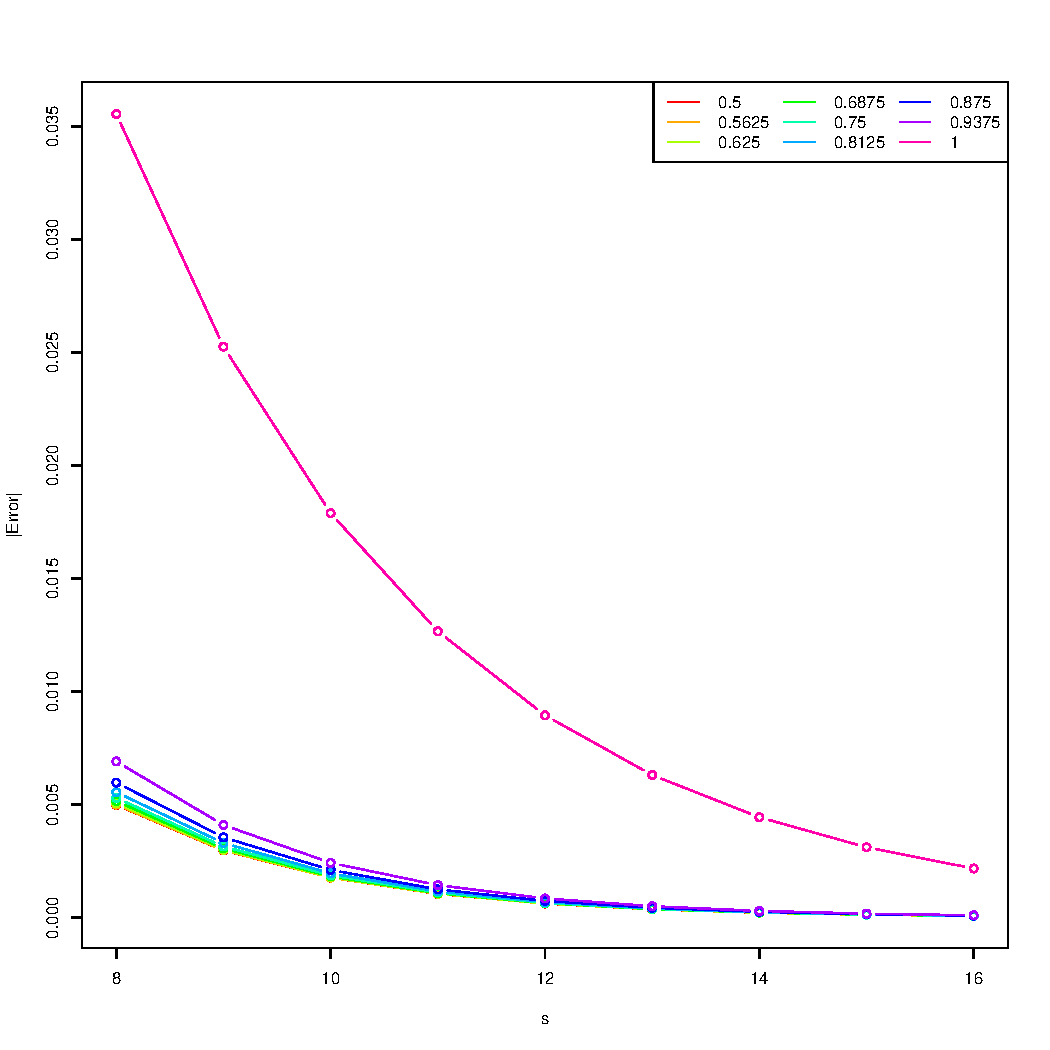
\includegraphics[scale=0.8]{nout_0a.pdf}
   \caption{Expectation of the absolute discretization error for selected $\alpha$-quantiles ($\alpha = 0.5, 0.5625, \cdots, 1$) using the Euler scheme with $N = 2^s$ ($4\le s \le 16$), $\mu=0$, $\sigma=1$, $T=1$, $X_0=0$ and $L=500000$. }
\label{f:ab}
\end{figure}
 
 \begin{figure}[p]
    %\centering
   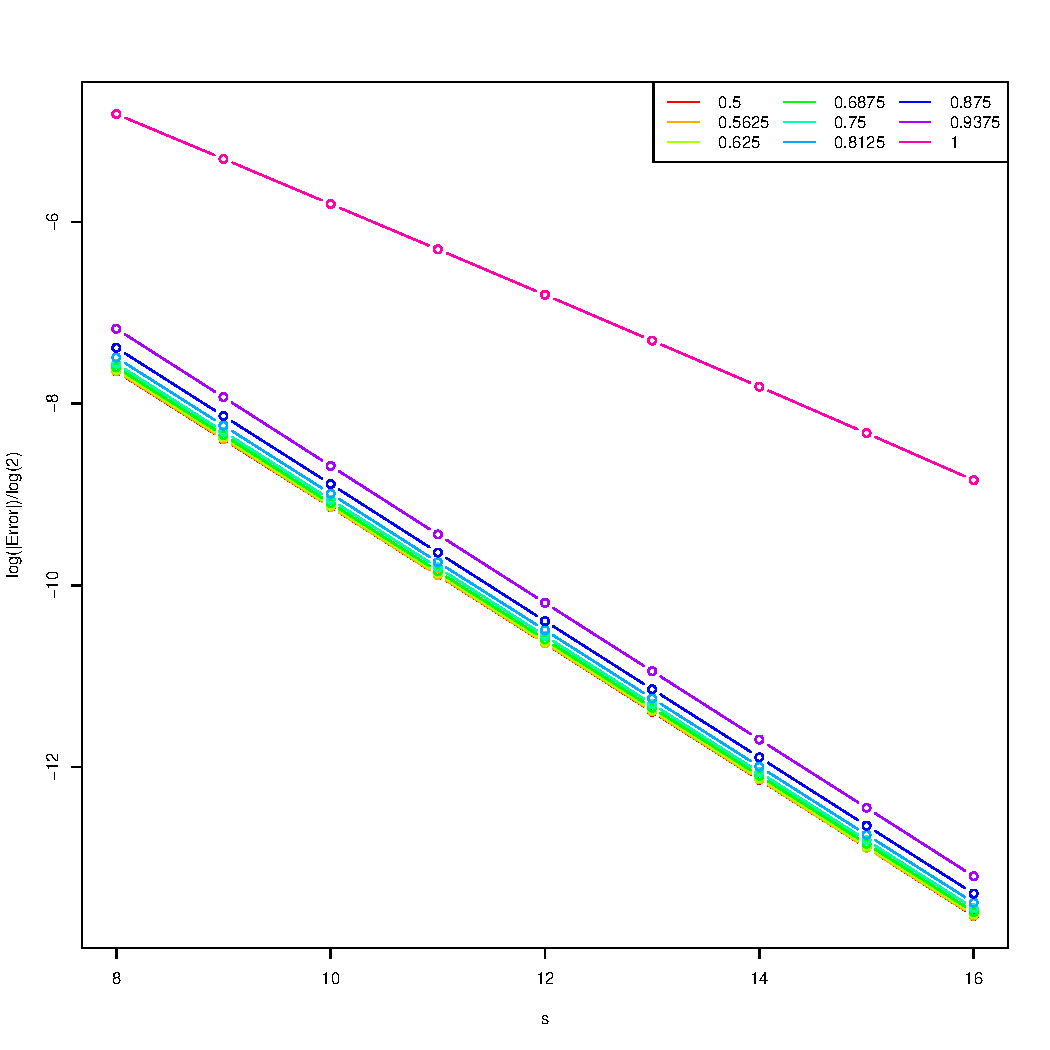
\includegraphics[scale=0.8]{nout_0alog.pdf}
   \caption{Logarithm of the absolute discretization error for selected $\alpha$-quantiles ($\alpha = 0.5, 0.5625, \cdots, 1$) using the Euler scheme with $N = 2^s$ ($4\le s \le 16$), $\mu=0$, $\sigma=1$, $T=1$, $X_0=0$, $L=500000$.} 
   \label{f:lab}
\end{figure}
 
 \begin{figure}[p]
   %\centering
   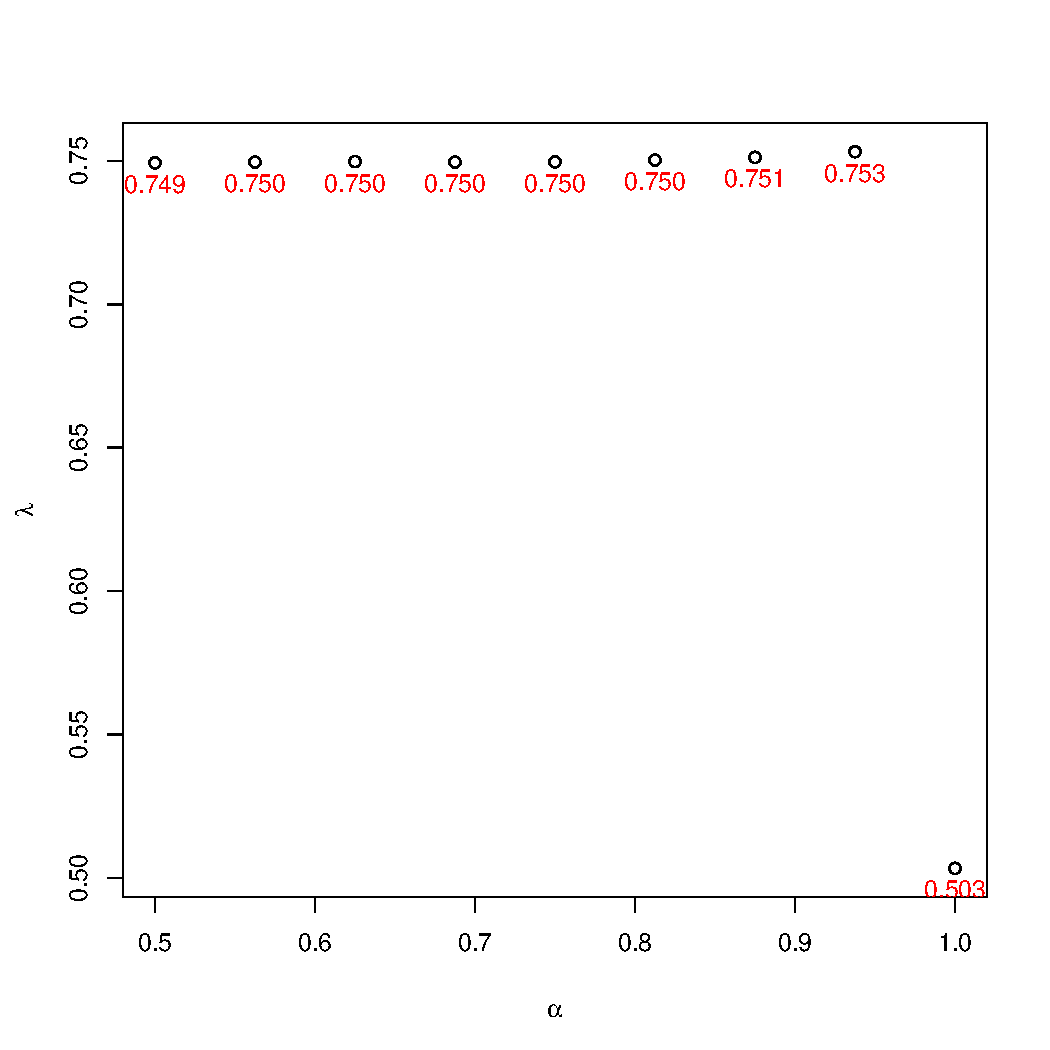
\includegraphics[scale=0.8]{nout_0arato.pdf} % requires the graphicx packagem 
   \caption{The strong order of convergence for selected $\alpha$-quantiles ($\alpha $ $=$ $ 0.5,$ $0.5625,$ $\cdots, 1$) using the Euler scheme with $N = 2^s$ ($4\le s \le 16$), $\mu=0$, $\sigma=1$, $T=1$, $X_0=0$, $L=500000$.}
   \label{f:ratio}
\end{figure}

% mu=0
\begin{figure}[p]
   %\centering
   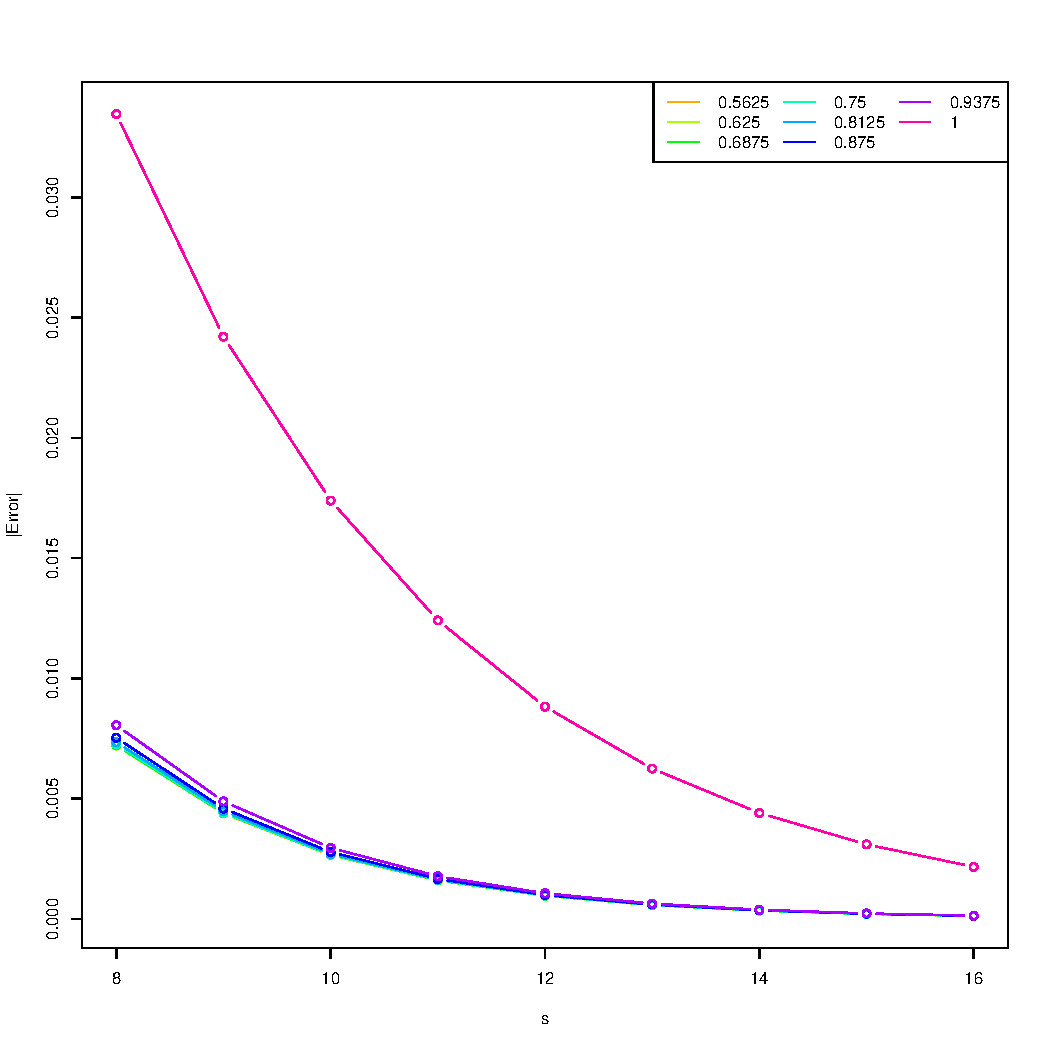
\includegraphics[scale=0.8]{nout_4_25_3a.pdf}
   \caption{Expectation of the absolute discretization error for selected $\alpha$-quantiles ($\alpha = 0.5, 0.5625, \cdots, 1$) using the Euler scheme with $N = 2^s$ ($4\le s \le 16$), $\mu=3$, $\sigma=1$, $T=1$, $X_0=0$, $L=500000$. }
\label{f:ab3}
\end{figure}
 
 \begin{figure}[p]
    %\centering
   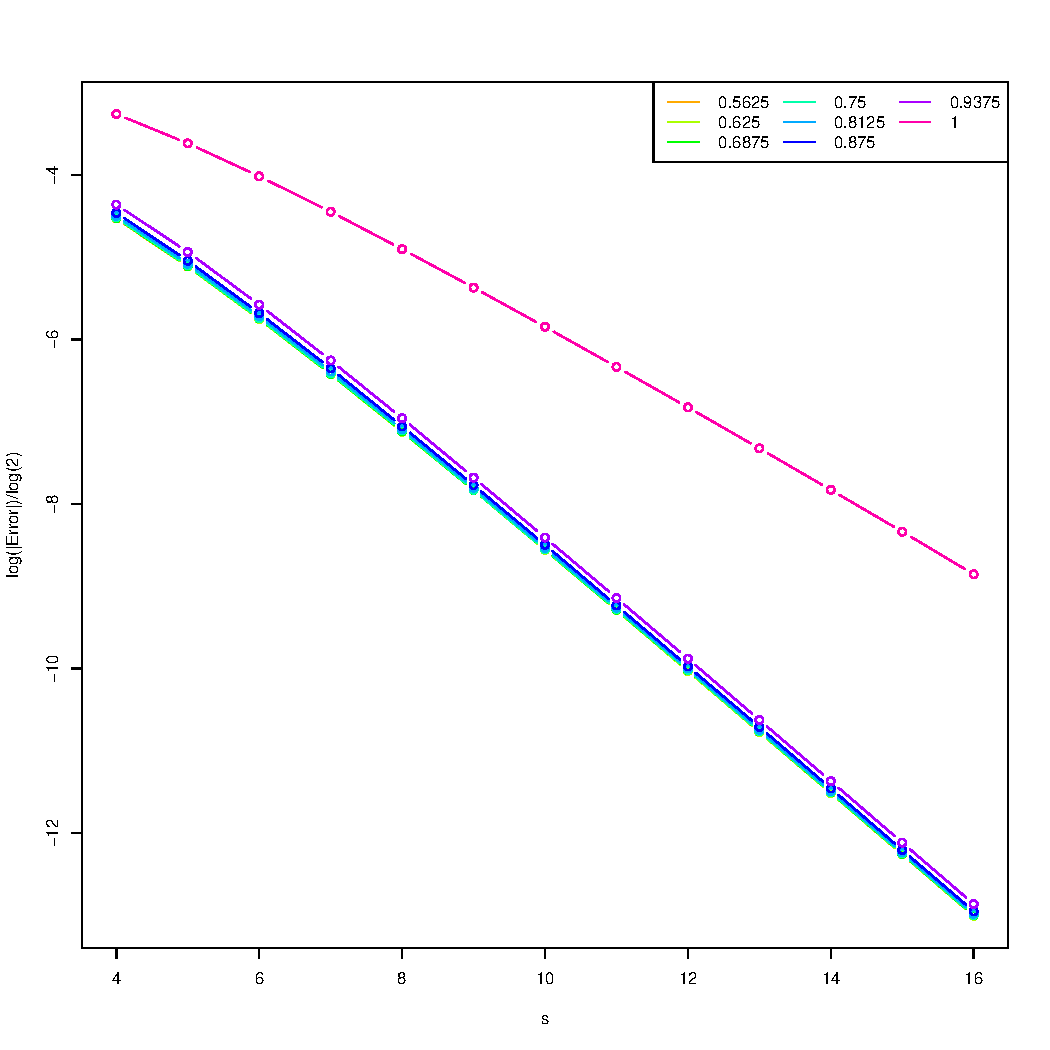
\includegraphics[scale=0.8]{nout_4_25_3alog.pdf}
   \caption{Logarithm of the absolute discretization error for selected $\alpha$-quantiles ($\alpha = 0.5, 0.5625, \cdots, 1$) using the Euler scheme with $N = 2^s$ ($4\le s \le 16$), $\mu=3$, $\sigma=1$, $T=1$, $X_0=0$, $L=500000$.} 
   \label{f:lab3}
\end{figure}
 
 \begin{figure}[p]
   %\centering
   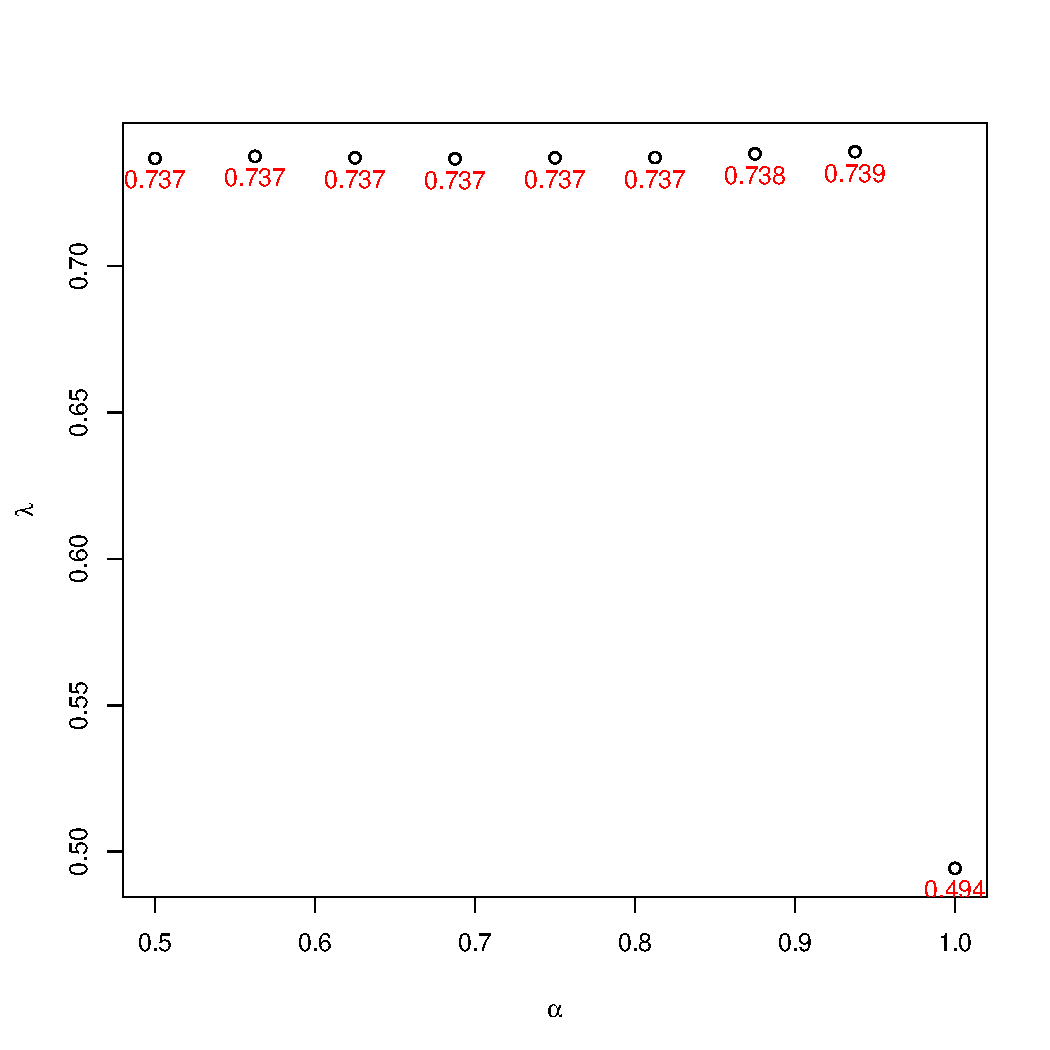
\includegraphics[scale=0.8]{nout_4_25_3arato.pdf} % requires the graphicx packagem 
   \caption{The strong order of convergence for selected $\alpha$-quantiles ($\alpha = 0.5, 0.5625, \cdots, 1$) using the Euler scheme with $N = 2^s$ ($4\le s \le 16$), $\mu=3$, $\sigma=1$, $T=1$, $X_0=0$, $L=500000$.}
   \label{f:ratio3}
\end{figure}

Although approximated strong order of convergence for $\mu=0$ and $\mu=3$ are not exactly the same, 
the convergence patterns are similar. 
As we expected, the strong order of convergence for the maximum is around $1/2$.
Moreover, for other quantiles, the strong order of convergence is far away from $1/2$, all of them are around to $0.75$.
These simulations reflect the huge difference of strong order of convergence for genuine quantiles and the maximum of a Brownian motion.
%It should be noticed, from these figures, it is hard to draw a conclusion of the role of $\mu$.
%We saw, a slight drift or the rato(\ref{f:ratio}\ref{f:ratio3}). We guess, the strong order of convergence will be decreeing when $\mu$ increase. 
%A "explanation" of this phenomenon is that when $\mu$ increase, the deterministic factor
%becomes more important and the random factor becomes weaker. 
%Since the discretization  error comes from the random part, it will decrease. 

\subsection{An analysis of the discretization error}
\label{sec:de}

%Let $X_k$ be a random walk (assume $X_0=0$)
%with i.i.d increment, i.e.
%$\Delta X_k = X_k -  X_{k-1}$ is i.i.d.
%Define the ordered statistics $M_{k,n}$ be the $k$-th smallest value in
%$\Set{X_i}_{i=0}^n$.
%Under this setting, clearly, $M_{0,n} = \inf_{0\leq i\leq n}X_i$
%and $M_{n,n} = \sup_{0\leq i\leq n}X_i$
%Define
%\[X'_i = X_{i+k}-X_k\]
%for fixed $k, n$.

%In \cite{Wendel1960}, an identity about random walk with
%i.i.d increment was derived:
%\begin{equation}\label{eq:dpathdec}
%(M_{k,n}, X_n) \eqlaw (\sup_{i\leq k} X_i +\inf_{i\leq n-k} X'_i, X_n).
%\end{equation}

%In \cite{Chaumont1999}, the author provided a combinatory treatment.
%He constructed a explicit path transform for $S$ to $\tS$, such that
%\[
%(M_{k,n}, S_n) = (\sup_{i\leq k} \tS_i+\inf_{i\leq n-k} \tS'_i, \tS_n)
%\]
%Here $\tS$ has same distribution with $S$ and each path $S$
% one-one correspondence to $\tS$.

%By using path transform, in \cite{Chaumont1999}, they proved
%following continuous version of path decomposition
%\begin{equation}\label{eq:cpathdec}
%(M_{\alpha,T}, X_T) \eqlaw (\sup_{t\leq \alpha{T}} X_t +\inf_{t \leq (1-\alpha)T} X'_t, X_T),
%\end{equation}
%where
%\[
%X'_t = X_{\alpha T+t} - X_{\alpha_T}.
%\]

%For the Brownian motion case, this formula were proved in many different ways
%and original due to \cite{Dassios1995}.


%\cite{Janssen2008} provided an estimate of the difference of expectations
%between the maximum of a Brownian motion and that associated with Gaussian random walks.
%Since we just give a really rough estimate, we only list the first two terms.
%For $W_t$ a Brownian motion with drift $\mu$ and variance $1$ on time interval $[0,1]$, that is $W_t = \mu t + B_t$, where $B_t$ is a standard Brownian motion, from \cite{Janssen2008} we get
%\begin{equation}\label{eq:est1}
%E\max_{0\leq t \leq 1} W(t) - E\max_{n=0,\cdots, N}W(n/N)
%= -\frac{\zeta(1/2)}{\sqrt{2\pi N}}-\frac{2g(1)-\mu}{4N} + O(1/N^{3/2}),
%\end{equation}
%where
%\[
%g(t) = \mu \Phi(\mu \sqrt{t}) + \frac{1}{\sqrt{2\pi t}} e^{-\frac{1}{2}\mu^2 t},
%\]
%and
%\[
%\zeta(1/2) \approx -3.92264613.
%\]
%\def\tW{\widetilde{W}}

%For general Brownian $\tW(t)$ motion on time interval $[0,T]$ with drift $\tmu$, variance $\tsigma$,
%we use following transform
%\begin{align*}
%\tW_t &= \tsigma \sqrt{T}W_{t/T} = \tsigma \sqrt{T} \mu t/T
%+ \sqrt{T}\tsigma B_{t/T},\\
%\mu &= \tmu \sqrt{T}/\tsigma.
%\end{align*}

%\def\tg{\widetilde{g}}
%We denote
%\begin{equation}
%\tg(\mu)=\mu \Phi(\mu) + \frac{1}{\sqrt{2\pi}} e^{-{1/2}\mu^2 }.
%\end{equation}

%We derive the following formula:
%\begin{equation}\label{eq:maxest}
%\begin{split}
%&E\max_{0\leq t\leq T} \tW(t) - E \max_{0\leq n \leq N} \tW(nT/N)\\ 
%= & -\frac{\zeta(1/2)}{\sqrt{2\pi}}\tsigma \sqrt{T/N}
% -\frac{2\tg(\mu)-\tmu\sqrt{T} / \tsigma}{4N}\tsigma\sqrt{T} +
%O(\sqrt{T}/N^{3/2}).
%\end{split}
%\end{equation}

In this section we provide a theoretical analysis about the expectation of the discretization error of the Euler approximation for $\alpha$-quantiles. We find that the leading order of the expectation of the discretization error \[\displaystyle E\varepsilon_N = \EE {M(\alpha,T) - \M(k,N)}\] is $1$ for $0 < \alpha<1/2$ or $0<\alpha<1/2$. That is the expectation of the discretization error is $O(1/N)$ when $0 < \alpha<1/2$ or $0<\alpha<1/2$. When $\alpha=1/2$, $E\varepsilon_N =0$. When $\alpha=1$ or $\alpha=0$, the expected discretization error is $O(1/N^{1/2})$ 

Combine $(\ref{eq:Dassios})$ $(\ref{eq:dpathdec})$ and $(\ref{eq:maxest})$, for $0 < \alpha < 1$,
we get an estimate of the expectation of the discretization error:
\allowdisplaybreaks
\begin{equation}\label{ex-dis-err-1}
\begin{split}
&\EE {M(\alpha,T) -  \M(k,N)}\\
=& \EE{\sup_{t\leq \alpha{T}} X_t +\inf_{t \leq (1-\alpha)T}X'_t} - \EE{\sup_{i\leq k} X_i+\inf_{i\leq N-k} X'_i}\\
=& \EE{\sup_{t\leq \alpha{T}} X_t +\inf_{t \leq (1-\alpha)T}X'_t
-  \sup_{i\leq k} X_i-\inf_{i\leq N-k} X'_i} \\
=&   \EE{\sup_{t\leq \alpha{T}} X_t - \sup_{i\leq k} X_i} +
\EE{\inf_{t \leq (1-\alpha)T} X'_t-\inf_{i\leq N-k} X'_i}\\
=& \EE{\sup_{t\leq \alpha{T}} X_t - \sup_{i\leq k} X_i} +
\EE{-\sup_{t \leq (1-\alpha)T} (-X'_t)+\sup_{i\leq N-k} (-X'_i)}\\
=& -\frac{\zeta(1/2)}{\sqrt{2\pi}}\sigma \sqrt{\frac{\alpha T}{\alpha N}} - \frac{2g(\mu_1)-\mu_1}{4\alpha N}\sigma\sqrt{\alpha T} +O(1/N^{{3}/{2}}) \\
&-\left(-\frac{\zeta(1/2)}{\sqrt{2\pi}}\sigma \sqrt{\frac{(1-\alpha)T}{(1-\alpha)N}} - \frac{2g(\mu_2) - \mu_2}{4(1-\alpha)N}\sigma \sqrt{(1-\alpha)T} + O(1/N^{{3}/{2}})\right) \\
=& -\frac{\zeta(1/2) \sigma}{\sqrt{2\pi}}\left(\sqrt{T/N} - \sqrt{T/N} \right)\\
& - \frac{\sigma\sqrt{T}}{4N}\left(\frac{(2g(\mu_1)-\mu_1)}{\sqrt\alpha} - \frac{(2g(\mu_2)-\mu_2)}{\sqrt{(1-\alpha)}}\right) \\
&+ O(1/N^{{3}/{2}}) \\
=&\frac{\sigma\sqrt{T}}{4N}\left(\frac{(\mu_1 - 2g(\mu_1))}{\sqrt\alpha} - \frac{(\mu_2 - 2g(\mu_2))}{\sqrt{(1-\alpha)}}\right) \\
& + O(1/N^{{3}/{2}}),
\end{split}
\end{equation}
where $k = \alpha N$, $\mu_1 =\mu\sqrt{\alpha T}/\sigma$, and $\mu_2 =-\mu\sqrt{(1-\alpha)T}/\sigma$.
The fourth last equality holds by view $\displaystyle\inf_{t\leq (1-\alpha)T} S'_t$ as
$\displaystyle-\max_{t\leq (1-\alpha)T} (-S'_t)$. 

Denote the coefficient of the leading term 
\[
\frac{\sigma\sqrt{T}}{4}\left(\frac{(\mu_1 - 2g(\mu_1))}{\sqrt\alpha} - \frac{(\mu_2 - 2g(\mu_2))}{\sqrt{(1-\alpha)}}\right)\]
as $\widetilde c(\mu,\alpha)$. In Figure \ref{plot-mu}, we can see the influence of $\mu$ and $\alpha$ on the coefficient of the leading term $\widetilde c(\mu,\alpha)$. Fixed $\mu$, we find that the closer $\alpha$ is to $1/2$, the closer $c(\mu,\alpha)$ is to $0$. Fixed $\alpha$, we find that the larger the value of $\mu$ is, the closer $\widetilde c(\mu,\alpha)$ is to $0$.

\begin{figure}[p]
   %\centering
   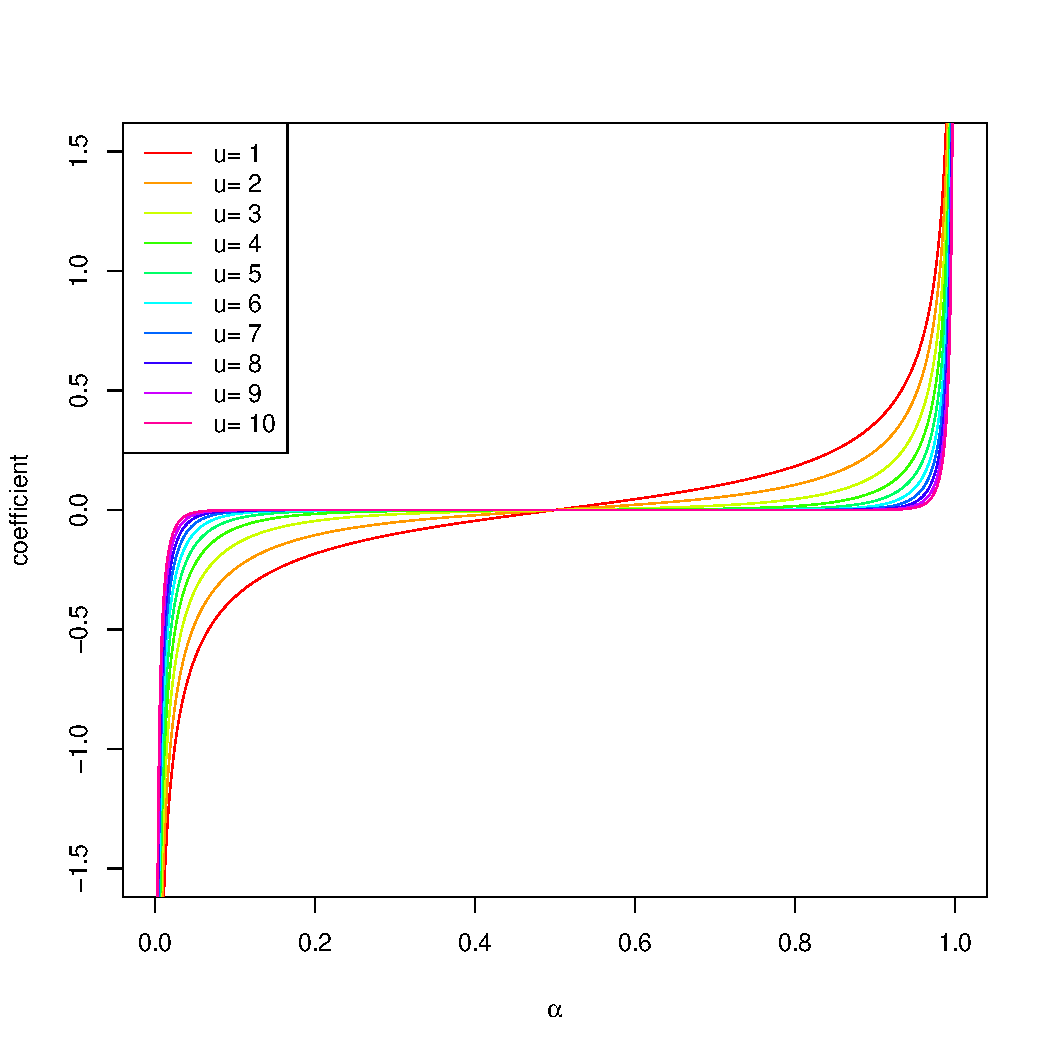
\includegraphics[scale=0.8]{mu.pdf} % requires the graphicx packagem 
   \caption{Coefficient of the leading term}
   \label{plot-mu}
\end{figure}


Since the discretization error for the maximum is axisymmetric with respect to $\mu=0$ (Section~\ref{s:euler}), we find that 
\begin{equation}\label{a-symmetric-alpha}
\begin{split}
&\EE{M(1-\alpha,T) - \M(N-k,N)} \\
=&\EE{\sup_{t\leq(1- \alpha){T}} X_t - \sup_{i\leq N-k} X_i} -
\EE{\sup_{t \leq \alpha T} (-X'_t)-\sup_{i\leq k} (-X'_i)}\\
=&\EE{\sup_{t\leq(1- \alpha){T}}(- X_t )- \sup_{i\leq N-k}(-X_i)}
-\EE{\sup_{t \leq \alpha T} (X'_t)-\sup_{i\leq k} (X'_i)}\\
=&-\left(\EE{\sup_{t \leq \alpha T} (X'_t)-\sup_{i\leq k} (X'_i)} - \EE{\sup_{t\leq(1- \alpha){T}}(- X_t )- \sup_{i\leq N-k}- (X_i)}
  \right)\\
=&-\EE {M(\alpha,T) -  \M(k,N)}.
\end{split}
\end{equation}
Equation (\ref{a-symmetric-alpha}) indicates that the expectation of discretization errors for $\alpha$-quantiles are  
central symmetric with respect to $\alpha=1/2$ when other parameters are fixed. 

We notice that when $\alpha=0.5$, the expected discretization error for the medium of a Brownian motion is 
\begin{equation}\label{ex-dis-err-2}
\begin{split}
&\EE {M(0.5,T) - \M(N/2,N)}\\
=& \EE{\sup_{t\leq 0.5{T}} X_t - \sup_{i\leq N/2} X_i} +
\EE{\inf_{t \leq (1-0.5)T} X'_t - \inf_{i\leq N/2} X'_i}\\
=& \EE{\sup_{t\leq 0.5{T}} X_t - \sup_{i\leq N/2} X_i} +
\EE{-\sup_{t \leq 0.5T} (-X'_t)+\sup_{i\leq N/2} (-X'_i)}\\ 
=& \EE{\sup_{t\leq 0.5{T}} X_t - \sup_{i\leq N/2} X_i} -
\EE{\sup_{t \leq 0.5T} (-X'_t) - \sup_{i\leq N/2} (-X'_i)}\\ 
=&0.
\end{split}
\end{equation}
The last equation holds because the expected discretization error of the maximum of a Brownian motion is axisymmetric with respect to $\mu =0$. 

From equation (\ref{ex-dis-err-1}), (\ref{ex-dis-err-2}) and result in \cite{A-G-P-1995}, we find that the order of the expectation of the discretization error for $\alpha$-quantiles of Brownian motion can be classified into three groups. When $\alpha=0$ or $\alpha=1$, \cite{A-G-P-1995} shows that the expectation of the discretization error for $\alpha$-quantile is $O(1/N^{1/2})$; when $0<\alpha<1/2$ or $1/2<\alpha<1$, equation (\ref{ex-dis-err-1}) shows that the expectation of the discretization error for $\alpha$-quantile is $O(1/N)$; when $\alpha=1/2$, equation (\ref{ex-dis-err-2}) shows that the expectation of the discretization error for $0.5$-quantile is $0$. 

%This proof shows that the expectation of the discretization error is $O(N^{-1})$ when $0<\alpha < 1$. When $\alpha = 0$ or $\alpha = 1$, the expectation of the discretization error is $O(N^{1/2})$. This partially explains the phenomenon related with the strong order of convergence we discussed in section \ref{s:euler}.   %If $\alpha=1/2$ and the Brownian motion does not have  drift ($\mu=0$), it is easy to see (by noting that $\E M_{1/2,T} = \E -M_{1/2,T}$) $\E M_{1/2,T} = \E M_{k,N} = 0$.When the Brownian motion has drift, the order becomes $1$.

The algorithm in section \ref{strong-order-convergence} is also able to analysis the expectation of the discretization error. The difference is that at the final stage of the algorithm, we average the sample value of the discretization error instead of the absolute value of the sample value of the discretization error. That is in the last step of the simulation algorithm we approximate the expectation of the discretization error for $s < d$ using:
\[
Err_{j,s} = \frac{1}{L}\sum_{1\leq l \leq L} \left({\M_{j,d}^{(l)}- \M_{j,s}^{(l)}}\right).
\]

We realize this algorithm for $d=25$, $b=4$, $\mu = 0$, $\sigma^2=1$, $T=1$, $X_0=0$ and generate $L=500000$ sampled paths. As you can see in Figure~\ref{f:err}, Figure \ref{f:lerr} and Figure \ref{f:rate}, the simulation results are coincident with our theoretical conclusions. 

Figure \ref{f:err3}, \ref{f:lerr3}, and \ref{f:rate3} depict the simulation results for $\mu=3$, $d=25$, $b=4$, $\mu = 0$, $\sigma^2=1$, $T=1$, $X_0=0$ and $L=500000$. As we can see from the figures, the convergence orders for genuine quantiles are all around $1$. 
Further more, we provide the comparison between the theoretical values and simulation results of coefficient of leading order $\log_2 (\widetilde c(\mu,\alpha))$ in Table~\ref{t:int0} and Table~\ref{t:int3}. We can see that they match pretty well. 

{\it Remark:} The reader may notice that lines wave much heavily for $\alpha$ closed to $0.5$ 
than $\alpha$ closed to $1$ in Figure~\ref{f:lerr} and Figure~\ref{f:lerr3}. Moreover, lines in Figure~\ref{f:lerr} 
are much smoother than those in Figure~\ref{f:lerr3}. This can be explained by Figure~\ref{plot-mu}.
As we can seen, $\widetilde c(\mu,\alpha)$ decreased dramatically when $\alpha$ is closing $0.5$ or the absolute value of $\mu$ is increasing.  
Noticing that  $\widetilde c(\mu,\alpha)$ controls the discretization error for fixed $N$, 
so the results are more sensitive to the error introduced by simulation itself 
when $\widetilde c(\mu,\alpha)$ is smaller. The results will be better if we do more simulations
 and these trends had been observed when we compared the figures for different times of simulations. 
However these simulations are really time consuming. 

\begin{table}[p]
\caption{Theoretical value and simulation results of $\widetilde{c}(\mu,\alpha)$ for $\mu = 0$
    using the Euler scheme with $N = 2^s$ ($4\le s \le 16$), $\mu=0$, $\sigma=1$, $T=1$, $X_0=0$, $L=500000$}

\begin{center}
\begin{tabular}{c|rrrrrrr}
$\alpha$ & 0.5625 & 0.625 & 0.6875 & 0.75 & 0.8125 & 0.875 & 0.9375  \\
\hline
theoretical &  -4.811 & -3.767 & -3.104 & -2.568 & -2.062 & -1.51 & -0.756\\
simulation & -5.09 &-3.755 & -2.919 & -2.635 & -2.053 & -1.550 & -0.743\\
\end{tabular}
\end{center}
   \label{t:int0}
\end{table}%

\begin{table}[p]
\caption{Theoretical value and simulation results of $\widetilde{c}(\mu,\alpha)$ for $\mu = 3$
    using the Euler scheme with $N = 2^s$ ($4\le s \le 16$), $\mu=0$, $\sigma=1$, $T=1$, $X_0=0$, $L=500000$}

\begin{center}
\begin{tabular}{c|rrrrrrr}
$\alpha$ & 0.5625 & 0.625 & 0.6875 & 0.75 & 0.8125 & 0.875 & 0.9375  \\
\hline
theoretical & -8.013 & -6.838 & -5.962 & -5.135 & -4.262 & -3.259 & -1.932\\
simulation & -9.211 & -7.496 & -5.615 & -4.938 & -4.094 & -3.215 & -1.881 \\
\end{tabular}
\end{center}
   \label{t:int3}
\end{table}%


%Intersection
%LSM:
% -14.2044267  -4.4445560  -3.4480370  -2.9903514  -2.5229556  -2.0290304  -1.6101579  -0.8828173  -0.9283404

%Theortical:
%  -Inf -4.8115536 -3.7676486 -3.1046530 -2.5682136 -2.0627128 -1.5106792 -0.7566437        Inf
%
%


%Drift 0, sim=127052
\begin{figure}[p]
   \centering
   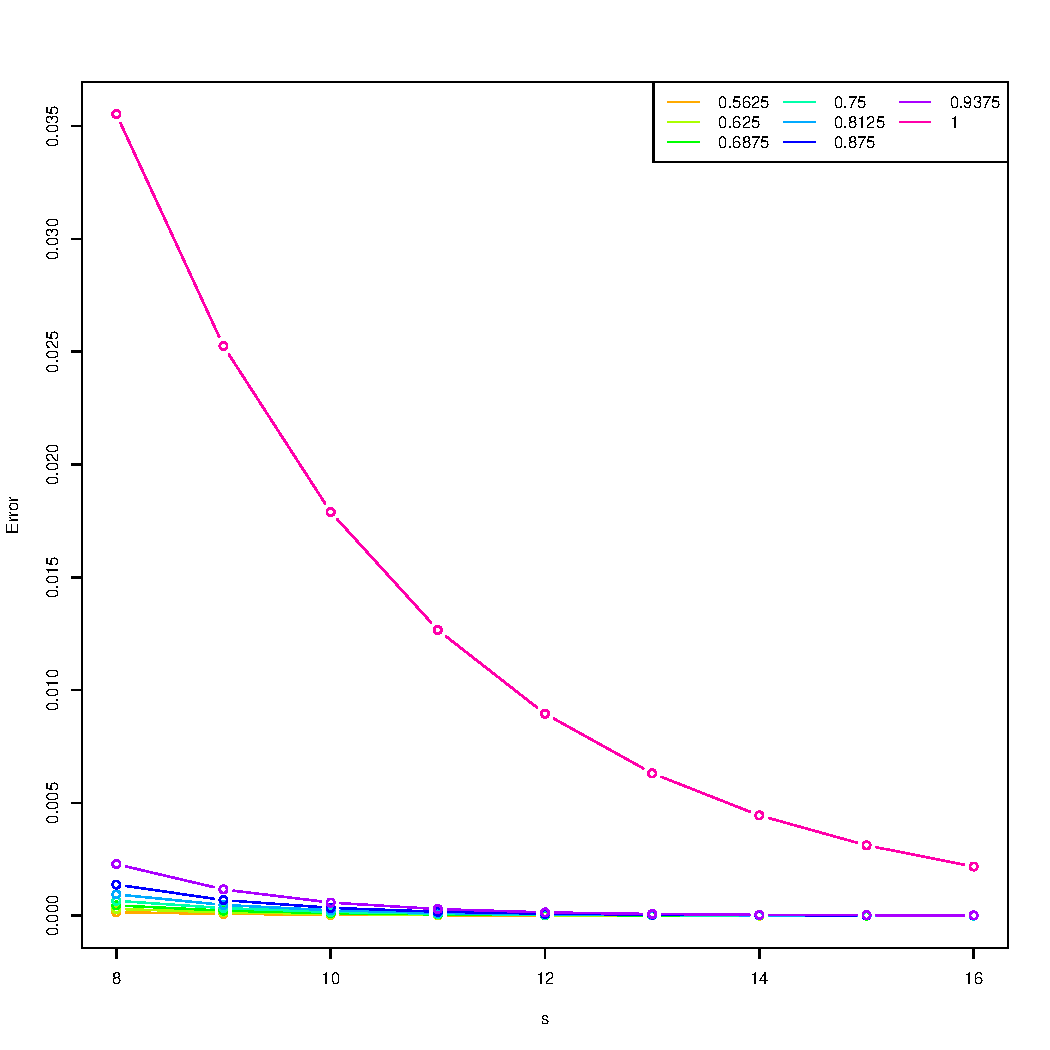
\includegraphics[scale=0.8]{nout_0.pdf} % requires the graphicx package
   \caption{Expectation of the discretization error for selected $\alpha$-quantile ($\alpha = 0.5625, 0.625, \cdots, 1$) using the Euler scheme with $N = 2^s$ ($4\le s \le 16$), $\mu=0$, $\sigma=1$, $T=1$, $X_0=0$, $L=500000$ }
   \label{f:err}
\end{figure}

\begin{figure}[p]
   \centering
   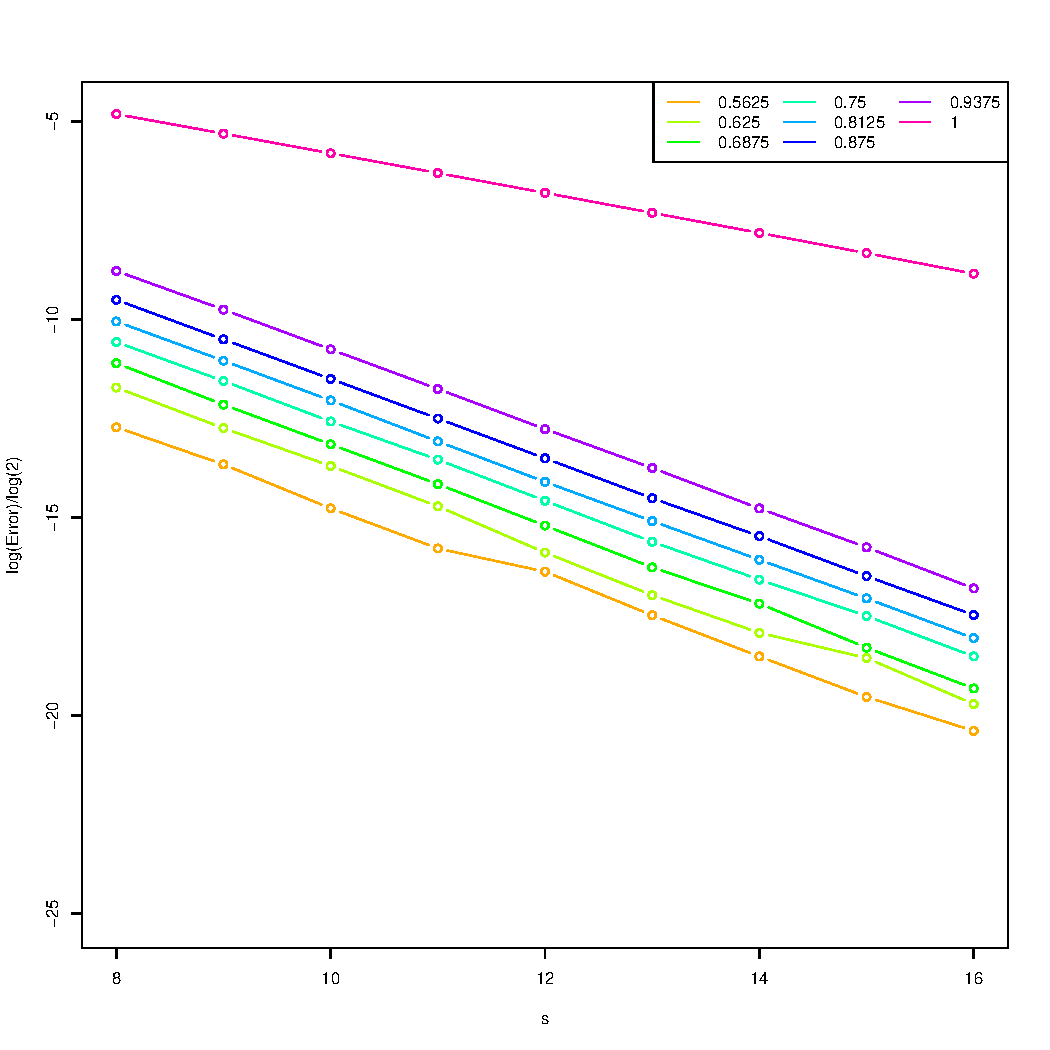
\includegraphics[scale=0.8]{nout_0log.pdf} % requires the graphicx package
   \caption{Logarithm of the discretization error for selected $\alpha$-quantile ($\alpha =$ $0.5625,$ $0.625,$ 
   $\cdots, 1$) using the Euler scheme with $N = 2^s$ ($4\le s \le 16$), $\mu=0$, $\sigma=1$, $T=1$, $X_0=0$, $L=500000$}
   \label{f:lerr}
\end{figure}

\begin{figure}[p]
   \centering
   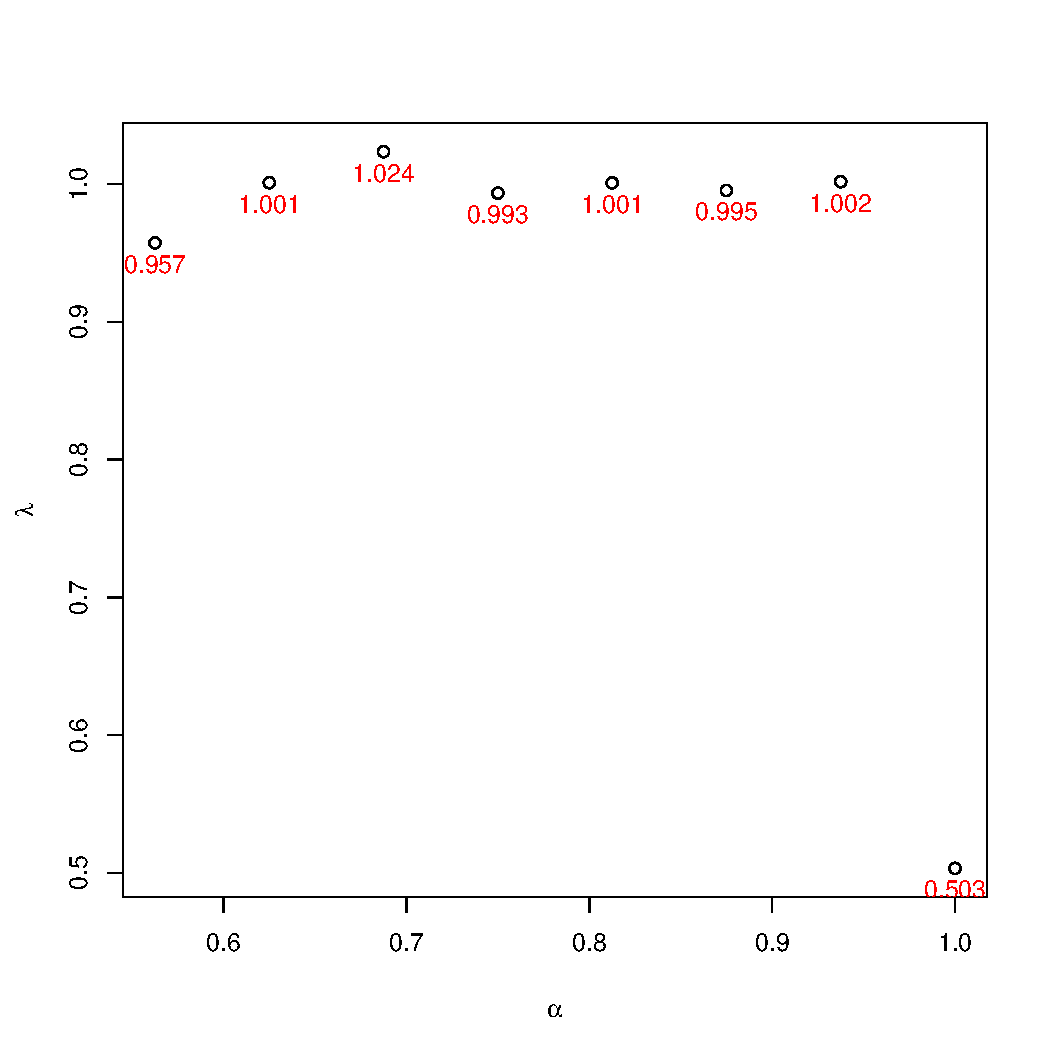
\includegraphics[scale=0.8]{nout_0rato.pdf} % requires the graphicx package
   \caption{The order of convergence for selected $\alpha$-quantile ($\alpha = 0.5625, 0.625,  \cdots, 1$) using the Euler scheme with $N = 2^s$ ($4\le s \le 16$), $\mu=0$, $\sigma=1$, $T=1$, $X_0=0$, $L=500000$}
   \label{f:rate}
\end{figure}

%Drift 0, sim=127052
\begin{figure}[p]
   \centering
   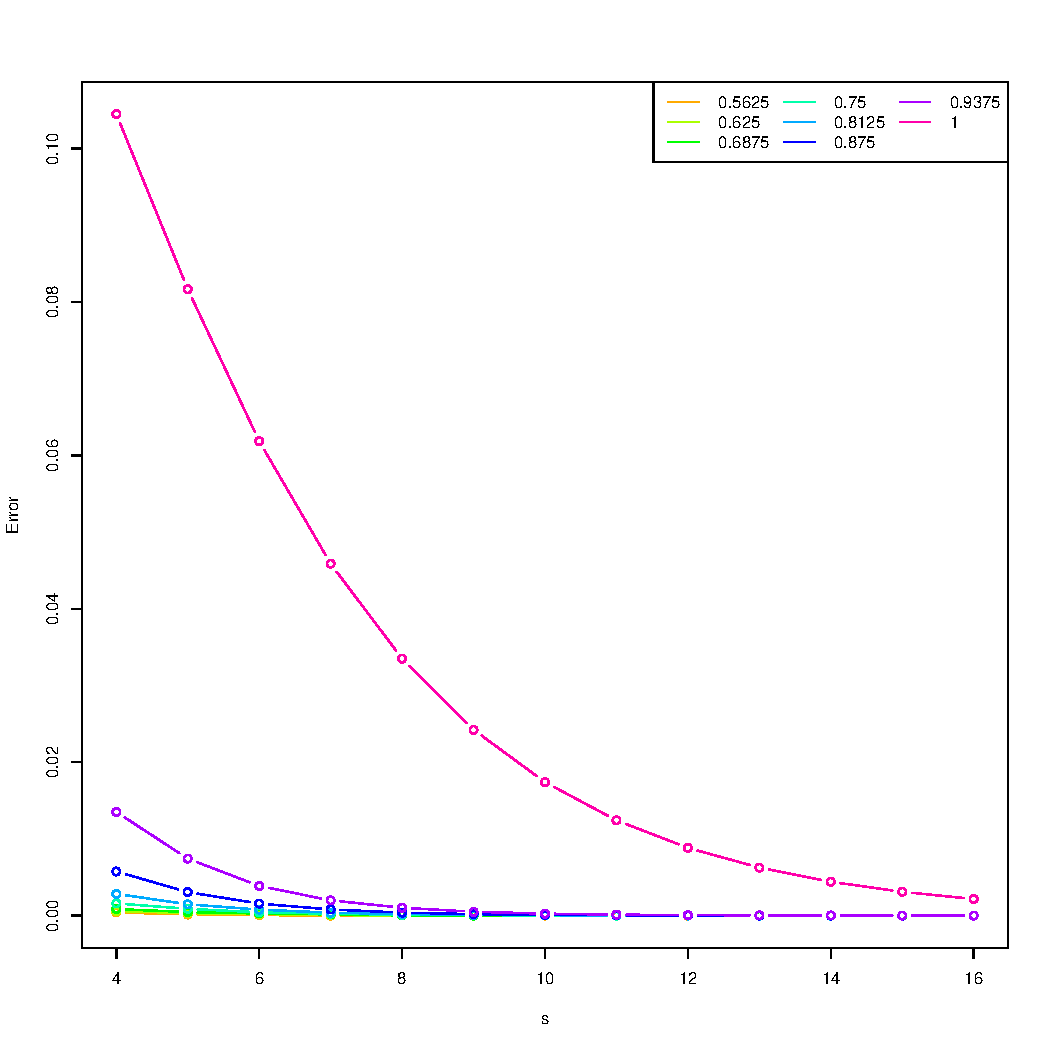
\includegraphics[scale=0.8]{nout_4_25_3.pdf} % requires the graphicx package
   \caption{Expectation of the discretization error for selected $\alpha$-quantile ($\alpha = 0.5625, 0.625,  \cdots, 1$) using the Euler scheme with $N = 2^s$ ($4\le s \le 16$), $\mu=3$, $\sigma=1$, $T=1$, $X_0=0$, $L=500000$ }
   \label{f:err3}
\end{figure}

\begin{figure}[p]
   \centering
   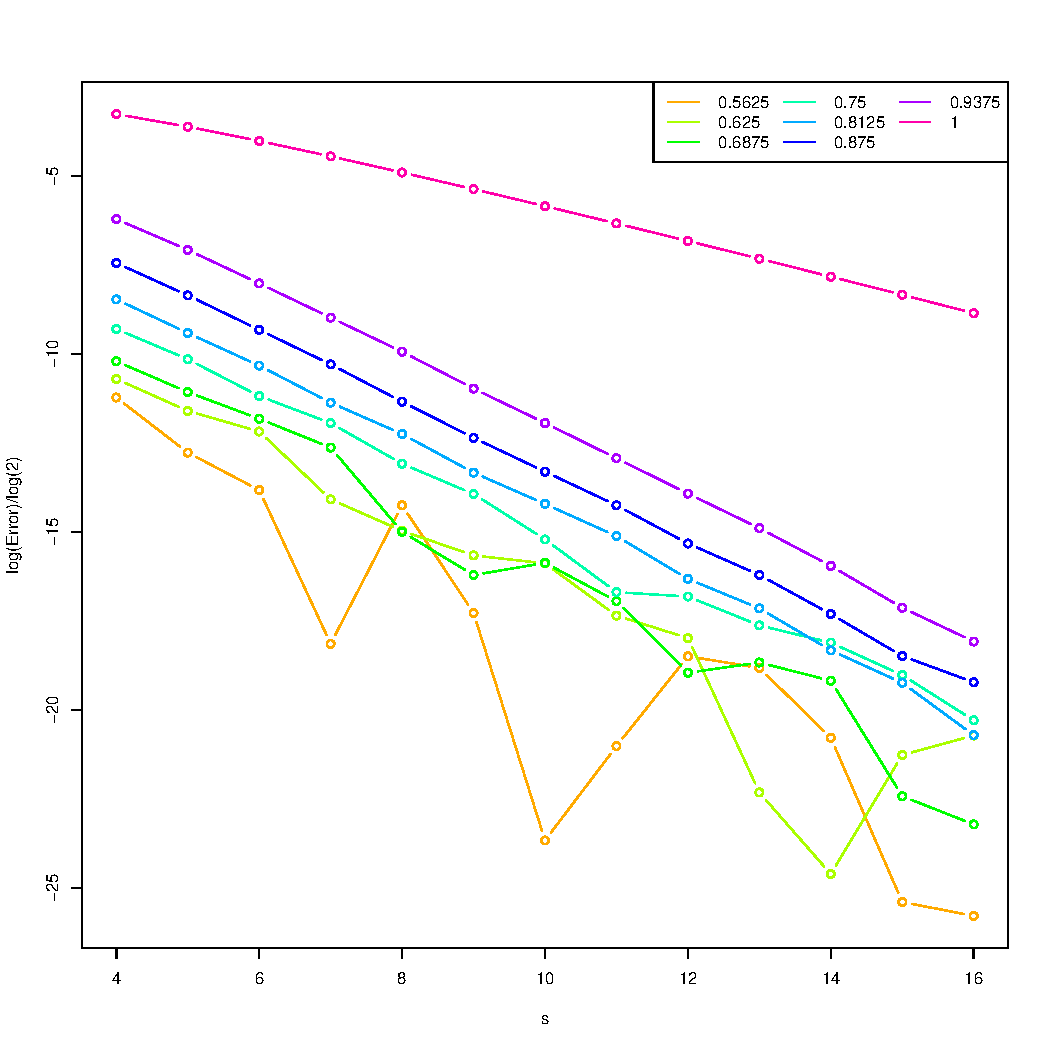
\includegraphics[scale=0.8]{nout_4_25_3log.pdf} % requires the graphicx package
   \caption{Logarithm of the discretization error for selected $\alpha$-quantile ($\alpha =$ $0.5625,$ $0.625,$  $\cdots, 1$) using the Euler scheme with $N = 2^s$ ($4\le s \le 16$), $\mu=3$, $\sigma=1$, $T=1$, $X_0=0$, $L=500000$}
   \label{f:lerr3}
\end{figure}

\begin{figure}[p]
   \centering
   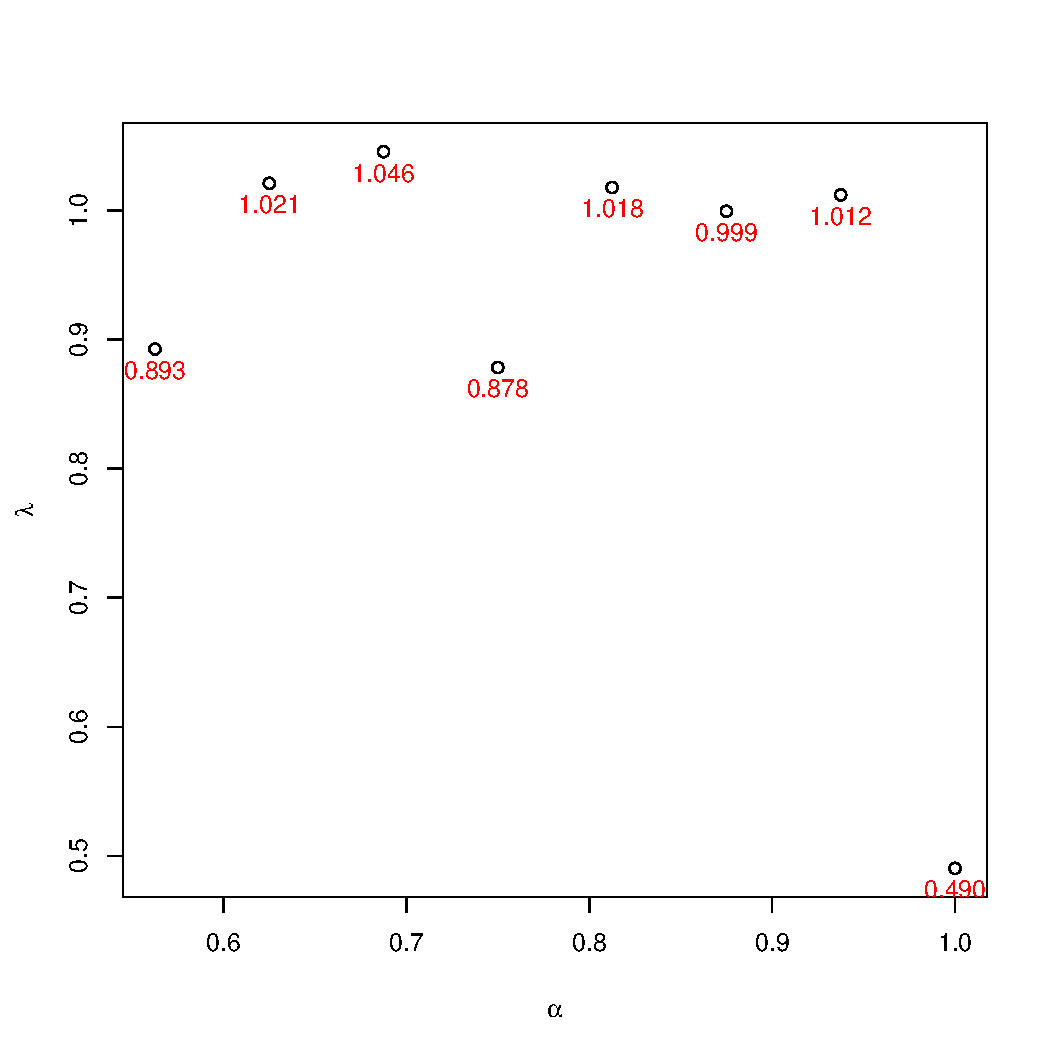
\includegraphics[scale=0.8]{nout_4_25_3rato.pdf} % requires the graphicx package
   \caption{The order of convergence for selected $\alpha$-quantile ($\alpha = 0.5625, \cdots, 1$) using the Euler scheme with $N = 2^s$ ($4\le s \le 16$), $\mu=3$, $\sigma=1$, $T=1$, $X_0=0$, $L=500000$}
   \label{f:rate3}
\end{figure}






%Now, suppose that $f$ is an monotone Lipschitz continuous function.Without loss of generality, assume 
%\begin{equation}\label{eq:lips}
%0 \leq f(x)-f(y) \leq C (x-y) \quad \forall x>y,
%\end{equation}
%for some constant $C$. This always is the case when $f$ is the
%(truncated) payoff of an $\alpha$-quantile option.

%Then it is easy to see
%\[
%-C\left( \sup_{t\leq (1-\alpha)T} (-S'_i)-\sup_{i\leq n-k} (-S'_i)\right)
% \leq f(M_{\alpha,T}) - f(M_{k,N})
%\leq  C \left(\sup_{t\leq \alpha{T}} S_t - \sup_{i\leq k} S_i\right)
%\]
%Hence
%\begin{equation}\label{eq:liperr}
%\abs{\E f(M_{\alpha,T}) - \E f(M_{k,N})}
%\leq \max\Set{\sqrt{\alpha}, \sqrt{1-\alpha}}
%C\frac{-\zeta(1/2)}{\sqrt{2\pi}}\sqrt{T/N}  + O(1/N)
%\end{equation}

%By this, we can say the convergence rate of $\alpha$-quantile European-style options at least 1/2.

\section{Quantile option}
\subsection{The advantage of quantile options}\label{4-3}
$\alpha$-quantile options, also known as quantile options, are a type of options whose payoff are functions of the quantiles of underlying asset price process. Firstly proposed in \cite{Miura}, the payoff function at maturity for a European-style $\alpha$-quantile call option with strike price $K$ and stock price at initiation $S_0$ is 
\begin{equation}
(S_0e^{M(\alpha,T)}-K)^+,
\end{equation}
and the payoff for a put option of this type is 
\begin{equation}
(K-S_0 e^{M(\alpha,T)})^+.
\end{equation}

As we discussed, the maximum and minimum of a process can be viewed as the extreme cases of the quantile when $\alpha=1$ and $\alpha=0$. Thus $\alpha$-quantile options are closely related to the lookback options. However, $\alpha$-quantile options have some advantages to lookback options. 

As we discussed before, the lookback option is a path-dependent option with payoff calculated with the maximum or minimum price of the underlying asset achieved during the life of the option. For example, a fixed strike lookback call option get the highest value obtained within the option's lifetime. In this case, to the holder, it can be viewed as a protection against large drop of stock price. This can be regarded as a method to deal with the unfavorable movement of a particular stock, such as the release of a prolonged lawsuit which may have a strong negative effect on the stock price. On the other side, a lookback put option provides an insurance against large rises. But these characters also make lookback options too expensive. An $\alpha$-quantile option is one product that overcomes this shortcoming of lookback options. A quantile option is cheaper than the lookback options with other identical variables, while it still provides partial protection against unfavorable market movements. This property of quantile options was first discussed by \cite{Ballotta2001}.

Another advantage of a quantile option is that the strong path dependence of its payoff makes it immunize to possible market manipulation. Because the payoff of a lookback option only involves the maximum or minimum of a stock price during the option's lifetime. Particularly for an at the money option close to maturity, which in this case are most vulnerable to the stock price movement closing to maturity. Firms have influence on market price can use this advantage to lead market price move to their favorable direction. But since a quantile option is strongly path-dependent, the manipulation effect is limited.

As for the pricing of quantile options, \cite{Dassios1995} provided the pricing formula for the European-style $\alpha$-quantile call option. However, it is expressed in form of a triple improper integral which brings computational difficulty to realize the price numerically. Inspired by the decomposition (\ref{eq:Dassios}), \cite{Laura2001} proposed a Monte Carlo simulation approach to value the price of a European-style $\alpha$-quantile option. \cite{Kwok2001} proposed a special way to apply tree method to price quantile options. In that paper, they find a relation between the price of quantile options and the price of cumulative Parisian options. By this approximation, they can simplify the pricing of quantile options. The detail of this method is provided in Appendix. However, both of these two numerical approaches only can get the initiation price at time $t=0$. In addition, both methods can not be extended to price American-style quantile options. In section (\ref{American-tree}), we propose a tree method which is capable to price both European-style and American-style ${\alpha}$-quantile options at any time $t\in [0,T]$ before maturity. 


\subsection{A tree method to price American-style quantile options}\label{American-tree}
Non-Markovian property of the quantile of a Brownian motion causes serious problem 
when we want to use tree method. We have to record all the information along the
path.% at least, we have to record the occupation time of $X_k$.
 
In risk-neutral world, we always can write the price of an
American-style quantile option in following way:
\[
V(S,\alpha,t;K) = \sup_{\tau\leq T} E[e^{-r(\tau-t))}f(S_0 M(\alpha, \tau);K)|\mathcal F_t],
\]
where $\tau$ are any stopping time stops taking value in $[t,T]$, $\mathcal F_t$ is the filtration contains all the information about stock price up to time $t$ and the payoff function
\[
f(x;K) = 
\begin{cases}
(x-K)^+ & \text{for call option},\\
(K-x)^+ & \text{for put option}.
\end{cases}
\]
This is an optimal stopping problem. 

The obvious way to solve this numerically, is using tree method. 
Discretize the time, i.e. let $0=t_0< t_1, \cdots, t_N =T$. Let $P_k=(X_0, \cdots, X_k)$ be a path in a binomial tree approximating the movements of a Geometric Brownian motion till time ${t_k}$. 
Then the possible value of the immediate next node $X_{k+1}$ along path $P_k$ can only be $X_{k}e^u$ and $X_{k}e^d$ with probability $p^+$ and $p^-$, where $u$, $d$, $p^+$ and $p^-$ are prefixed constants in the usual binomial tree method. We denote the two possible paths one step longer than path $P_k$ as $P_k^+ = (X_0,\cdots,X_k,X_{k+1}=X_{k}e^u)$ and $P_k^- = (X_0,\cdots,X_k,X_{k+1}=X_{k}e^d)$. 
Then let 
\[
\mathrm{Pay}_{P_k} = f(X_{P_k}^\alpha;K)
\] 
be the payoff if the option holder exercise the option at time $t_k$, 
where $X_{P_k}^\alpha$ denotes the $\alpha$-quantile of path $P_k$. 

Due to the early exercise right of an American-style option, the price of the American-style $\alpha$-quantile option along path $P_k$ at time $t_k$ for $k<N$ should be 
\begin{equation}\label{AM-V-1}
V_{P_k} = \max\Set{E_{P_k}, \mathrm{Pay}_{P_k}},
\end{equation}
where
\begin{equation}\label{AM-V-2}
E_{P_k} = e^{-r(t_{j+1}-t_j)}(p^+V_{P_k^+} + p^-V_{P_k^-})
\end{equation}
is the option value if we choose to keep the option instead of exercising it at $t_k$ along path $P_k$. 

At the end of path $P_N=(X_0, \cdots, X_N)$, i.e, at maturity, the price of an option should be the immediate payoff. Then the option price corresponding to path ${P_N}$ at time $t_N$ 
\begin{equation}\label{AM-V-3}
V_{P_N} = \mathrm{Pay}_{P_N}.
\end{equation}
%For $j< n$, 
%let 
%\[
%C_{P_j} = \max\Set{E_{P_j}, \mathrm{Pay}_{P_j}}
%\]
%where
%\[
%E_{P_j} = e^{-r(t_{j+1}-t_j)}(p^+C_{(P_j,X_j+u)} + p^-C_{(P_j,X_j-d)})
%\]
%is the expectation return if the holder of the option
%do not exercise his right at time $t_j$, providing the historical data of 
%the stock price is given by $P_j$. 

By the recurrence relation in (\ref{AM-V-1}) (\ref{AM-V-2}) and the final condition in (\ref{AM-V-3}), we can compute the price of an American-style $\alpha$-quantile option at time $t_0$.

Now the optimal stopping time is given by 
\[
\tau(P_n) = \inf\Set{t_j| Pay_{P_j}\geq E_{P_j}},
\]
here $P_j$ is the restriction of $P_n$ at $(t_0, \cdots, t_j)$, i.e. 
\[
P_j = (X_0, \cdots, X_j) \quad \text{ if } P_n=(X_0, \cdots, X_n). 
\] 

Because of the non-Markovian attribute of $\alpha$-quantile of a process, the tree we applied to price American-style quantile option is not recombining. We illustrate how our tree looks like in Figure (\ref{fig-bitree}). In Figure (\ref{fig-bitree}), we present a tree with depth $3$. Node $0$ is called the root of the tree and nodes $8,\cdots,15$ are called the leaves of this tree. Nodes $4$ and $5$ are the two children of node $2$, while node $2$ is the parent of node $4$ and $5$. 

It is nature to realize the pricing algorithm by using the ``Depth First Search'' algorithm. Depth first search (DFS) is a standard algorithm for visiting all nodes and generating all possible paths in a tree. The character of this method is that we start from the root of a tree and explore as deep as possible until the end of each branch before backtracking. In practice, we build the tree with depth $N$, each non-leaves node $X_j$ has two children corresponding to $\Set{X_j e^u,X_j e^d}$. Hence the computational complexity of this ``brute force'' method is $O(2^n)$. It is clear that all the nodes at depth $j$ correspond to one and only one path $P_j$. So we label the node by $ND_{P_j}$.  For any node, say $ND_{P_j}$, we first compute $E_{P_{j}}$, where the possible $ND_{P_{j+1}}$ are all of its two children. After visiting all its children and computing the two possible $V_{P_{j+1}}$, it backtracks to node $N_{P_j}$, and computes $E_{P_j}, Pay_{P_j}$ and then $V_{P_j}$. After that, it goes back to the parent of $N_{P_j}$. Now we apply the same process to $N_{P_{j-1}}$  as we do to $N_{P_{j}}$. In other words, if it does not finish visiting all its children, it will visit the next one; if it finishes visiting all the children, it will compute the value of the node and goes back to its parent. 


\begin{figure}[p]
   \centering
   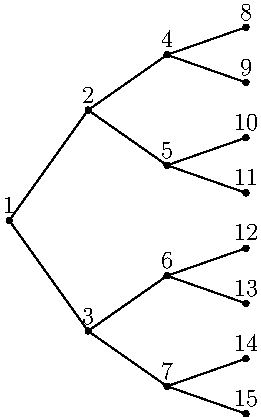
\includegraphics{bitree.pdf} % requires the graphicx package
   \caption{A tree to price American-style $\alpha$-quantile options}
   \label{fig-bitree}
\end{figure}

We know that there is no other method to price American-style $\alpha$-quantile options so far. In other words, there does not exist direct result acting as a comparing standard. However, since conceptually our tree should also work for European-style $\alpha$-quantile options, here we first compare the price of European-style quantile options from our tree method with value obtained by other methods.

The results with parameters 
\[
K=100, r=0.05, \sigma=0.2, \alpha=0.5, T=1, 
\]
can be seen in Table~\ref{fig:euro5}. It took 6 hours to get the price of American-style quantile option at a tree with 36 steps at High Performance Computer with Intel Xeon 3.00GHz CPU.



\begin{table}[p]
\caption{The price of European-style $\alpha$-quantile call options, with parameters
	$K=100, r=5\%, \sigma=0.2, \alpha=0.5, T=1$. }
	%The extrapolation is based on results got at 28 steps and 36 steps. Data for paper is from \cite{Laura2001}.
\begin{center}
\begin{tabular}{l|lllllll}
 $S_0$ & $90$ & $95$ & $100$ & $105$ \\
\hline
28 steps & 1.60216 & 3.17876 & 5.61323 & 8.92661\\
30 steps & 1.60443 & 3.17806 & 5.61404 & 8.92702\\
32 steps & 1.60637 & 3.18346 & 5.61678 & 8.92718\\ 
34 steps & 1.60435 & 3.18426 & 5.61758 & 8.92875\\
36 steps & 1.60411 & 3.18846 & 5.61940 & 8.92925\\
%\hline
%Extrapolation & 1.61094 & 3.22241 & 5.64100 & 8.938490 \\
%\hline
%Paper & 1.6588 & 3.2695 & 5.7501 & 9.0895\\
\hline
Monte Carlo & 1.62450 & 3.21390 &  5.65385 & 8.96801 \\
Standard error & 0.00141 & 0.00200 & 0.00262 & 0.00317 \\
\hline
lookback & 9.45696 & 13.86499 & 19.16763 & 24.88215
\end{tabular}
\end{center}
\label{fig:euro5}
\end{table}%

In Table~\ref{fig:euro8}, for parameters set as $\alpha = 0.8$, $K = 95$, $r = 5\%$, $\sigma = 20\%$, and $T = 0.25$, we present the results got by our tree method and Forward Shooting Grid discussed in section \ref{se:fsg}.

\begin{table}[p]
\caption{The price of European-style $\alpha$-quantile call options,
	with parameters
	$K=95, r=5\%, \sigma=0.2, \alpha=0.8, T=0.25$. }
	%The extrapolation is based on results got at 28 steps and 36 steps.
\begin{center}
\begin{tabular}{l|lllllll}
$S_0$ & $95$ & $100$ & $105$        \\
\hline
26 steps & 4.59876 & 9.10824 & 14.1838 \\
28 steps & 4.60931 & 9.11777 & 14.1954 \\
30 steps & 4.61547 & 9.12485 & 14.2030 \\
32 steps & 4.61816 & 9.12648 & 14.2054 \\
34 steps & 4.61785 & 9.12676 & 14.2051 \\
36 steps & 4.62050 & 9.12908 & 14.2079 \\
%extrapolation & 4.659665 & 9.168665 & 14.25165\\
\hline
FSG & 4.66082 & 9.16298 & 14.2309 \\
\hline
Monte Carlo & 4.66740 & 9.18266 & 14.26175\\
Standard error & 0.00168 & 0.00200 &  0.00214\\
\hline
lookback & 8.381566 &  13.76059 & 19.13961
\end{tabular}
\end{center}
\label{fig:euro8}
\end{table}%


\begin{table}[p]
\caption{The price of American-style $\alpha$-quantile call options, with parameter
	$K=100, r=0.05, \sigma=0.2, \alpha=0.5, T=1$. 
	%The extrapolation is based on results got at 28 steps and 36 steps.
	}
\begin{center}
\begin{tabular}{l|lllllll}
$S_0$ & $90$ & $95$ & $100$ & $105$ \\
\hline
26steps & 1.69411 & 3.43582 & 6.19546 & 10.2276 \\
28steps & 1.70066 & 3.44695 & 6.21365 & 10.2465 \\
30steps & 1.70434 & 3.45157 & 6.22887 & 10.2624 \\
32steps & 1.70651 & 3.45927 & 6.24320 & 10.2738 \\
34steps & 1.70590 & 3.46373 & 6.25529 & 10.2831 \\
36steps & 1.70711 & 3.47019 & 6.26644 & 10.2891 \\
%Extrapolation & 1.729685 & 3.551530 & 6.451205 & 10.43820 \\
\end{tabular}
\end{center}
\label{fig:amer5}
\end{table}%

\begin{table}[p]
\caption{The price of American-style $\alpha$-quantile call options, with parameters
	$K=95, r=5\%, \sigma=0.2, \alpha=0.8, T=0.25$. 
	%The extrapolation is based on results got at 28 steps and 36 steps.
	}
\begin{center}
\begin{tabular}{l|lllllll}
$S_0$ & $95$ & $100$ & $105$        \\
\hline
26 & 4.84702 &  9.68628 & 14.8771\\
28 & 4.85892 &  9.70169 & 14.8932\\
30 & 4.86696 &  9.71225 & 14.9049\\
32 & 4.87621 &  9.72318 & 14.9164\\
34 & 4.88228 &  9.73134 & 14.9251\\
36 & 4.88821 &  9.73857 & 14.9329\\
%extrapolation & 4.990725 & 9.867650&  15.07185
\end{tabular}
\end{center}
\label{fig:amer8}
\end{table}%


Comparing the results by our tree method with Forward shooting grid and the Monte Carlo method, we think our tree method is correct. Since, as we checked, it works well for European-style $\alpha$-quantile options, it should also work for American-style $\alpha$-quantile option. The Monte Carlo method we adapted is resorting to the decomposition of the $\alpha$-quantile of a Brownian motion (\ref{eq:Dassios}). Different with the method proposed in \cite{Laura2001}, we simulate the maximum of a Brownian motion proposed in \cite{A-G-P-1995}. All the results for this Monte Carlo method is based on $10,000,000$ paths. The related standard errors are also reported. 


For parameters set as
\[
K=100, r=0.05, \sigma=0.2, \alpha=0.5, T=1,
\]
with our tree method, we present the price of American-style $\alpha$-quantile call options in Table \ref{fig:amer5}. Comparing data in Table \ref{fig:euro5} and Table \ref{fig:amer5}, we can see American-style $\alpha$-quantile call options are more expensive than European-style options with same feature. This again insures that our method is correct. 

For parameters set as 
\[
K = 95,\alpha = 0.8, r = 5\%, \sigma = 20\%, T = 0.2,
\]
comparing the American-style $\alpha$-quantile options price in Table \ref{fig:amer8} and the price for the European-style options of this type in Table \ref{fig:euro8}, we find that our tree method gives the right relation between these two styles of options.

We also observe that in Figure \ref{fig:euro5} and \ref{fig:euro8}, in the European case, quantile options are cheaper than the lookback options. This feature makes quantile options meet the needs of a larger group of investors. 

\subsection{An extrapolation method to improve the accuracy of our tree method}
Because the computational time of this method is going exponentially as the steps increasing. It is very time consuming to obtain an result with large steps. To solve this question, we propose an extrapolation method to improve the accuracy of the price for quantile options based on our tree method. 

Richardson extrapolation is a method to accelerate the sequence convergence rate first studied by \cite{Richardson}.
Let $v(h)$ be the approximate price of the option got from the tree method with step length $h$. Suppose the tree method is of order $\vartheta$.  
We have 
\[
v(h) = v_0 + Ch^\vartheta + O(h^{\vartheta'}),
\]
where $v_0$ is the true value of the $\alpha$-quantile option and $\vartheta' > \vartheta$ .
Then for two different step length $h_1, h_2$ we have 
\begin{equation}\label{v(h-1)}
v(h_1) = v_0 + Ch_1^\vartheta + O(h_1^{\vartheta'}),
\end{equation}
and
\begin{equation}
v(h_2) = v_0 + Ch_2^\vartheta + O(h_2^{\vartheta'}).
\end{equation}
Let $\eta = h_1/h_2$, we have 
\begin{equation}\label{v(h_2)}
v(h_2) = v\left(\frac{h1}{\eta}\right) = v_0 + C\left(\frac{h1}{\eta}\right)^\vartheta + O(h_1^{\vartheta'}). 
\end{equation}
Multiplying (\ref{v(h_2)}) by ${\eta}^\vartheta$ we have 
\begin{equation}\label{v(h-2-v)}
{\eta}^\vartheta v\left(\frac{h_1}{\eta}\right) = {\eta}^\vartheta v_0 + Ch_1^\vartheta + O(h_1^{\vartheta'}).
\end{equation}

Subtracting (\ref{v(h-2-v)}) by (\ref{v(h-1)}),
we get 
\begin{equation}\label{v-1-eta}
{\eta}^\vartheta v\left(\frac{h_1}{\eta}\right) - v(h_1) = v_0({\eta}^\vartheta  -1) + O(h_1^{\vartheta'}).
\end{equation}
From (\ref{v-1-eta}), we get 
\begin{equation}
v_0= \frac{{\eta}^\vartheta v({h_1}/{\eta}) - v(h_1)}{{\eta}^\vartheta -1} + O(h_1^{\vartheta'})
\end{equation}
which gives a higher order ${\vartheta}'$ approximation for $v_0$. 
%we get
%\[
%v_0(h_1^\vartheta - h_2^\vartheta) \approx h_1^\vartheta v(h_2) - h_2^\vartheta v(h_1)
%\]
%i.e. 
%\[
%v_0 \approx \frac{ h_1^\vartheta v(h_2) - h_2^\vartheta v(h_1)}{
%  h_1^\vartheta - h_2^\vartheta}
%= \frac{\eta^\vartheta v(h_2) - v(h_1)}{\eta^\vartheta -1 },
%\]
%where $\eta = h_1/h_2$.

%In our case, denote $C_n$ be the value corresponding to a $n$-steps tree. Based on the conclusion in section \ref{sec:de}, it is reasonable to assume that our tree method converges on order 1. That is $\gamma = 1$. 
%Then the true value of $\alpha$-quantile option 
%\[
%C_\infty \approx \frac{\eta C_{n_2} - C_{n_1}}{\eta-1},
%\]
%where $\eta = (T/n_1)/(T/n_2) = n_2/n_1$.
%This is the general form of Richardson extrapolation.
%If take $n_2=2n, n_1=n$, we get the usual Richardson extrapolation formula
%\[
%C_\infty \approx 2 C_{2n} - C_n. 
%\]

To apply this method to our pricing problem, we need decide the extrapolation based on what order $\vartheta$ and which pair of price obtained from trees with different steps. Since the price of European-style $\alpha$-quantile options can be priced by the Monte Carlo simulation and conceptually our tree method also works for European-style $\alpha$-quantile options, we can apply the best fitted extrapolation method for European-style $\alpha$-quantile options to the identical American-style $\alpha$-quantile options. Suppose we get the price for a set of quantile options with $\{\alpha_i, i=1,\cdots,m\}$ and otherwise identical parameters using our tree method and extrapolation methods on various parameters. Denote $v_{(i,n1,n2,\vartheta)}$ as the price obtained from the extrapolation method based on the price got from a $n1$-step tree and $n2$-step tree and on order $\vartheta$ for European-style $\alpha$-quantile option with $\alpha=\alpha_i$. Denote $v^\infty_i$ as the price for the European-style $\alpha_i$-quantile option obtained by the Monte Carlo method. We use mean error 
\begin{equation}\label{mean-error}
\sum_{1\leq m} (v_{(i,n1,n2,\vartheta)} -v^\infty_i)^2 /m 
\end{equation}
as the criterion to measure the accuracy for the extrapolation method based on the price from $n1$-step and $n_2$-step trees and with order $\vartheta$. Then the best fitted extrapolation method is the extrapolation method which gives the minimum mean error (\ref{mean-error}) among extrapolation methods with order $\vartheta$ in a given set $\mathcal A$ and $(n1,n2)$ in a given set $\mathcal B$.  After finding the best set of parameters $(\widetilde n1, \widetilde n2, \widetilde\vartheta)$, we can apply this best fitted extrapolation method to the price of American-style $\alpha$-quantile options obtained from our tree method. 

We realize the extrapolation method to quantile options with parameters set as $S=100$, $K=100$, $r=5\%$, $\sigma=0.2$, $T=1$ and $\{\alpha = 0.5, 0.6, 0.7, 0.8, 0.9\}$. In this example the order $\vartheta$ lying in $\mathcal A = \{0.1, 0.2, \cdots, 2\}$ and $\{(n_1,n2)|n1<n2; n1=10, 11,\cdots, 36; n2= 10,11,\cdots, 36\}$. Our program shows that the best extrapolation approximation is based on $\vartheta = 0.9$ and price obtained from a $18$-steps tree and $36$-steps tree. We present the result in Table \ref{fig:euro9}. Apply this extrapolation approximation to the price for American quantile options from our tree method, we get Table \ref{fig:amerc}. From these two tables, we can see that both the price of European-style and American-style $\alpha$-quantile call options increases as the value of $\alpha$ increases. %One can observe that price of $\alpha$-quantile options are cheaper than lookback options constructed on identical market variables. This feature of $\alpha$-quantile options provide more choices to investors with various needs and perspectives of the market. 
 


\begin{table}[p]
\caption{The price of European-style $\alpha$-quantile call options, with parameters
	$S=100, K=100, r=5\%, \sigma=0.2, T=1$ and different $\alpha$. }
\begin{center}
\begin{tabular}{l|lllll}
$\alpha$ & $0.5$ & $0.6$ & $0.7$ & $0.8$ & $0.9$       \\
\hline
18 steps  & 5.58991 & 7.02836 & 8.64998 & 10.5450 & 12.9325\\
36 steps  & 5.61940 & 7.07069 & 8.70835 & 10.6295 & 13.0804\\
\hline
Extrapolation  & 5.65345  & 7.11957  & 8.77575 & 10.72707 &13.25117 \\
\hline
Monte Carlo & 5.65519 &7.11064 & 8.77318 & 10.73129 & 13.24507\\
Standard eror &  0.00262 & 0.00303 & 0.00344 & 0.00386 & 0.00430    
\end{tabular}
\end{center}
\label{fig:euro9}
\end{table}%


\begin{table}[p]
\caption{The price of American-style $\alpha$-quantile call options, with parameters
	$S=100, K=100, r=5\%, \sigma=0.2, T=1$ and different $\alpha$. }
\begin{center}
\begin{tabular}{l|lllllll}
$\alpha$ & $0.5$ & $0.6$ & $0.7$ & $0.8$ & $0.9$       \\
\hline
%26 & 6.19546 & 7.65852 & 9.26385 & 11.1028 & 13.3703\\
%28 & 6.21365 & 7.67208 & 9.2838 & 11.1237 & 13.3911\\
%30 & 6.22887 & 7.68475 & 9.29502 & 11.1397 & 13.4019\\
%32 & 6.2432 & 7.69856 & 9.3113 & 11.1572 & 13.4248\\
%34 & 6.25529 & 7.71023 & 9.32278 & 11.168 & 13.4488\\
18 steps & 6.10629 & 7.57527 & 9.16086 & 10.9735 & 13.1843\\
36 steps & 6.26644 & 7.72127 & 9.32848 & 11.1789 & 13.4651\\
\hline
Extrapolation & 6.451357 & 7.889848 & 9.522022 & 11.416064 & 13.789325 
\end{tabular}
\end{center}
\label{fig:amerc}
\end{table}%

\chapter{Conclusion and future work}
In this thesis, we provide a numerical study about the strong order of convergence of the Euler approximation associated with the simulation of the $\alpha$-quantile of Brownian motion. We find that the strong order of convergence for genuine $\alpha$-quantile of Brownian motion where $\alpha \in (0,1)$ is around $0.75$, while the strong order of convergence for the maximum or the minimum of Brownian motion is $0.5$.  Strong order can be used to connect the price of continuously and discretely monitored $\alpha$-quantile options in future work.  We provide an analysis about the expectation of the discretization error for the Euler approximation of the $\alpha$-quantile of Brownian motion, which shows that the order of the expected discretization error can be classified into three groups when $\alpha$ is at different level.

$\alpha$-quantile options, a type of strong path-dependent options, are discussed. Existing pricing methods (Monte Carlo method and forward shooting grid method) are only able to give the initiation price for European-style options of this type. We propose a tree method which can price both European-style and American-style $\alpha$-quantile options. Using the price of European-style $\alpha$-quantile options obtained from Monte Carlo method, we have shown how extrapolation method can be applied to improve the accuracy of our pricing method. Although we only discuss the pricing problem of the fixed-strike $\alpha$-quantile options, our tree method is also valid to price the floating-strike quantile options. We also notice that our tree can price the $\alpha$-quantile options at time $t$ after the initiation of a contract, since at time $t$ information about the stock price during $(0,t)$ is available.    

\appendix
\chapter{A forward shooting grid method for a European $\alpha$-quantile option}
\label{se:fsg}


Like lookback options, quantile options are also path-dependent. What makes things difficult is that the quantile of a process is not Markovian. Normal tree methods which usually involve backward induction do not work in this case. We need to record all the information of the path because of lack of Markovian property, which will lead the tree to explosion computationally.
\cite{Kwok2001} proposed a special way to apply tree method to price quantile options. In this paper, they find a relation between the price of quantile option and the price of cumulative Parisian option. By this approximation, they can simplify the pricing of quantile option. In their paper, they assume that there are $M$ time steps for the whole monitoring period $[0,T]$, and they define $S^M_j$, $j = - M$, ...$0$,$1$,...,$M$ as the set of all the possible value the asset prices value can be at maturity. Under trinomial tree method, the possible prices happened in one tree are limited to $S^M_j$,  $j = - M$, ...$0$,$1$, ...,$M$, which is also true for the value taken by the quantile of a stock price process $\{S_t\}, t \in[0,T]$. Therefore they derived that
\begin{equation}\label{eq:kowk1}
V(\alpha, T) = e^{-rT} \sum^{M}_{j=-M}P[S_0 M(\alpha,T)=S^{M}_{j}]\max(S^{M}_{j}-K,0),
\end{equation}
where $V(\alpha,T)$ is for the value of a  European-style fixed-strike $\alpha$-quantile option whose maturity is $T$, $P[S_0M(\alpha,T)=S^{M}_{j}]$ is the probability that the quantile of Brownian motion achieve the value $S^M_j$,  $j = - M$, ...$0$,$1$, ...,$M$. In their paper, they observed that the difference between the prices of two cumulative Parisian binary options is a good approximation for $P[S_0M(\alpha,T)=S^{M}_{j}]$ multiplies discount factor $e^{-rT}$, i.e.,
\begin{equation}\label{eq:kowk2}
\begin{split}
\displaystyle e^{-rT}P[S_0M(\alpha,T)&=S^{M}_{j}] \approx V^{bin}_{cum}[(1-\alpha)T, S^{M}_{j-1}]-V_{cum}^{bin}[(1-\alpha)T, S_{j}^{M}\\
&\quad\text{ for }j=-M, ... , 0, 1, ... , M
\end{split}
\end{equation}
where $V^{bin}_{cum}[d,B]$ is denoted as the price of continuously monitored cumulative Parisian binary option with down barrier $B$, and $d$ be the minimum cumulative time staying above the down barrier to avoid knock-out.


Combining equation (\ref{eq:kowk1})and (\ref{eq:kowk2}), they get
\begin{equation}\label{eq:kowk3}
V_{alp} = \sum^M_{j=-M} \max (S^M_j - K,0) \times \{V_{cum}^{bin}[(1-\alpha)T, S^M_{j-1}] - V^{bin}_{cum}[(1-\alpha)T, S^M_j]\} ,
\end{equation}
where $V^{bin}_{cum}[(1-\alpha)T, S_{-(M+1)}^M] = e^{-rT}$. By this result, they turn pricing of a quantile option into pricing of $2M+1$ cumulative Parisian options.


Parisian option is like an advanced version of barrier option. We know barrier options are options where the payoff depends on whether the underlying asset's price reaches a certain level (barrier) during the option's life. Barrier options usually trade in the over-the-counter market. This kind of options are attractive because they are usually cheaper than similar options without barrier. Like vanilla option, barrier options also authorize holders the right to buy or sell, but  long sides of barrier options do not need to pay for scenarios they think is unlikely to happen in the future. One good example I find from Wikipedia is about IBM. If you believe that IBM will go up this year, but are willing to bet that it will not go above \$100, then you can buy the barrier and pay fewer premium than the coresponding vanilla option. But in this one-touch knock-out or knock-in can bring difficulties to option writers when asset price is close to barrier, particularly, in market where manipulation of underlying asset price is not impossible. To overcome short period price manipulation, various adjustments to one-touch knock out or knock-in have been applied in practice. The Parisian options is one solution. In order to get activated, the underlying assets of a Parisian option need to stay in the knout out or knout in region for certain period of time. The payoff of a cumulative Parisian option is dependent on the total amount of time the underlying asset price has spent above or below barrier. As for a binary option, the payoff is either some fixed amount of some asset or nothing at all.


A forward shorting grid (FSG) has been proposed to price cumulative Parisian option in \cite{Kwok2001}. The character of FSG is that this approach need add additional information at each node of a lattice tree. Commonly in pricing path-dependent option, at each node we should add state vector to represent the path-dependent attribute, such as the extreme value of the underlying asset price achieved in the lookback option case. As we know \cite{Hull1993} and \cite{Vijh1993} were the first authors suggested this approach. \cite{Barraquand1996} introduced a comprehensive framework for FSG. In this paper they indicated that the FSG method is unconditionally convergent. %Further, they showed that when the covariance matrix is degenerate, the FSG method can outperform finite difference methods. 
The convergence of the FSG algorithm in pricing of Asian options was studied by \cite{Forsyth1999}.

In \cite{Kwok2001}, they constructed a trinomial tree to get the price of a cumulative Parisian option. But due to the fact that the result is not steady according to the setting of the length of up movement between each immediate step, we modify their method to binomial tree.

In building binomial tree, we start by cutting the entire life of one option into many small time intervals of length $h = T / N$.
Our tree is build to mimic the logarithm process of underlying asset price. Denote $s=\ln S$. In each step, the logarithm of the price of underlying asset is assumed to move from its initial value of $s_0$ to one of the two new values, $s_0 + d + u$ and $s_0 + d - u$ with equal probability, that is $p_{up} = p_{down} = 0.5$ , where $u = \sigma \sqrt{h}$ and $d = (r - {\sigma}^2 /2)h$. Here $\sigma$, and $r$ are volatility and risk-free interest rate, respectively. The model is illustrated in Figure~\ref{fig:tree1}.
\begin{figure}[p]
   \centering
   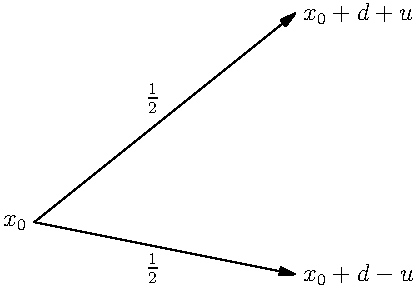
\includegraphics{trees.pdf} % requires the graphicx package
   \caption{Forward shooting}
   \label{fig:tree1}
\end{figure}

Like the notation used in \cite{Kwok2001}, we denote $V[m,j;k]$ as the numerical option value of the cumulative Parisian option at the $m$-th time interval,  $j$ upward jumps from the initial underlying asset value and $k$ times breaches so far. Let $g(k,j)$ be the grid function that describes the correlated evolution of number of breaches $k$ and price indicate $j$. Denote $s_j$ be the value of $s$ corresponding to $j$ upward movements on the binomial tree. Then we should add $1$ to the indicator $k$ if the underlying asset price $S$ is no more than the barrier $B$; i.e $s_j \leq \ln B$. Hence we can see that a suitable setting of the grid evolution function $g(k,j)$ should be
\begin{equation}\label{eq:grid}
g(k,j) = k + 1_{\Set{s_j \leq \ln B}}
\end{equation}
where $1_{\set{s_j \leq \ln B}}$ is the indicator function. It is defined as
\begin{equation}\label{eq:grid-indicator}
1_{\Set{s_j \leq \ln B}} =  \begin{cases}
1 & \text{if } s_j \leq \ln B \\
0 & \text{if } s_j > \ln B
\end{cases}
\end{equation}
Then the FSG method for pricing the cumulative Parisian binary option can be expressed as
\begin{equation}\label{eq:fsg}
V[m-1,j;k] =\set{0.5V[m,j+1;g(k,j+1)]+0.5V[m,j-1,g(k,j-1)]}e^{-rh}
\end{equation}
for $m-1 < N$.

Let $\widetilde N$ be the predetermined number of breaches recorded for the all duration of the life of an option that is desired to activate the contract.
Considering the binary feature of the option, we should initiate our algorithm with
\begin{equation}\label{eq:initiate}
V[M,j;k] = \begin {cases}
1 & \text{if }  k < \widetilde N\\
0 & \text{if }  k \geq \widetilde N.
\end{cases}
\end{equation}
By (\ref{eq:initiate}) , (\ref{eq:fsg}) and backward induction, we can get the price of cumulative Parisian binary option with any prescribed times of breaches and barrier.

Recall what we get by equation (\ref{eq:kowk2}). In order to get the price of $\alpha$-quantile option, we can use the prices of $2M + 1$ cumulative Parisian binary options to approximate $\alpha$-quantile option's value. Hence using the FSG method we described above to calculate the prices of cumulative Parisian option and doing a simple math work by equation (\ref{eq:kowk2}), we can get the approximated price for $\alpha$-quantile option with $M$ time steps.

Recall we defined earlier $h = T / M$. We compute the approximated option price of an $\alpha$-quantile call option with different time steps using equation (\ref{eq:kowk2}). As you can see in Figure (\ref{fig:2}),
the numerical values of option are plotted against varying $h$. The values of parameters of the $\alpha$-quantile call option are set as: $\alpha = 0.8$, $S_0 = 100$, $X = 95$, $r = 5\%$, $\sigma = 20\%$, and $T = 0.25$.
\begin{figure}[p]
   \centering
   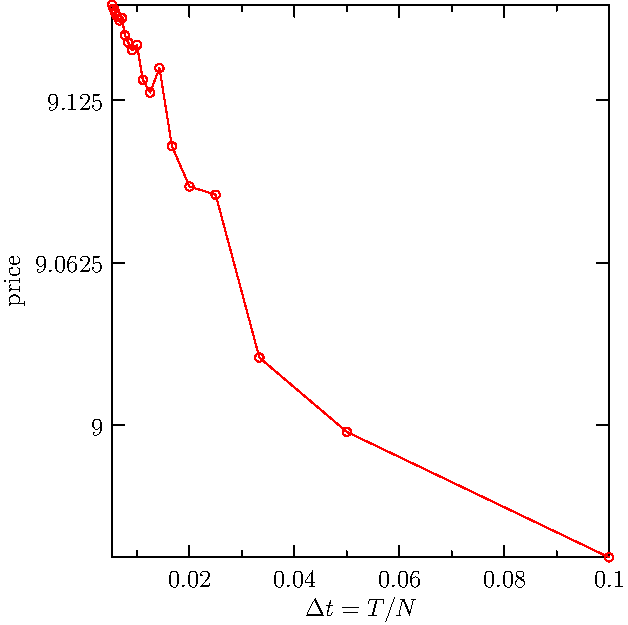
\includegraphics{bfsg.pdf} % requires the graphicx package
   \caption{FSG results}
   \label{fig:2}
\end{figure}




%\subsection{A static hedging for $\alpha$-quantile put option}
%Inspired by the approximation of quantile option using cumulative Parisian options, we here propose a static hedging of quantile options using cumulative binary Parisian options. As we discussed earlier, the payoff of a cumulative binary Parisian option is that: only if the price of stock spend enough time under a predetermined barrier, its payoff is \$1; otherwise, its payoff is 0, it is worth nothing. We explicitly account for the discreteness of the tick size. That is the value of stock price only can be multiples of 1/8. Then for a put quantile option, the intuition for our hedging lies in the ability to rephrase the question, what was the certain quantile of stock price as several questions. 

%For example, for $40\%$-quantile put option with stock price started from 1 and strike price 2, we can replicate its payoff using cumulative Parisian options which are alive only if they spend more than $0.4*T$ time under their barrier. For the quantile option, it has payoff only if the $40$ percentile is less than 2, the strike price. Also it is obvious that $40$ percentile must be larger than 0. In this sense, we hold 0.125 share of each cumulative binary Parisian binary option with barrier raging from $0.125. 0.250, 0.375.�, 2$.  If in the end of maturity, the 40 percentile of stock price is larger than 2, the quantile option gets nothing. Since the 40 percentile is larger than 2, then the stock price must be under 2 for less than 40$\%$ of the time before maturity. In this case all the binary option gets nothing. But if the quantile is $1.750$, the quantile option gets a payoff of $0.250=2-1.750$. While for the binary options, in this case, options with barrier $2$ and $1.875$ are alive. The payoff you can get from binary options is $0.125*2=0.250$. That is the payoff of the collections of binary options is identical to your quantile option. These are true for other scenarios of the value of quantile.  In other words, by holding a collection of cumulative Parisian binary option, we can realize a static hedging.

%Probably, you have already found out that this scheme only works for European puts, because that you can find the two side boundary of effective quantile. This condition is not true for calls. 



\bibliography{prob}

\end{document}  